\documentclass[10pt]{article} 
\usepackage{palatino} %times} %% USES MUCH LESS SPACE

\usepackage[usenames,dvipsnames]{color}
\usepackage{xspace}
\usepackage[font=bf,aboveskip=7pt,belowskip=-10pt]{caption} 
\usepackage{subfig}
\usepackage{soul}
\setlength{\oddsidemargin}{0in}
\setlength{\evensidemargin}{0in}
\setlength{\topmargin}{-0.6in}
\setlength{\textheight}{9.05in}
\setlength{\textwidth}{6.5in}

\usepackage[compact]{titlesec}
% The above line seems to be creating a pdflatex error.  [HG]
% SPACE

\usepackage{color}
\usepackage{cite}
\usepackage{verbatim}
\usepackage[hyphens]{url}

\usepackage{epsfig}
\usepackage{amssymb}
\usepackage{amsmath}
\usepackage{amsfonts}

\usepackage{slashbox}
\usepackage{graphicx}

%\usepackage[top=0.9in, bottom=0.9in, left=0.75in, right=0.75in]{geometry}
%\usepackage[T1]{fontenc}
%\usepackage{amsmath,  amsthm,  amssymb}
%\usepackage{amsmath,    amssymb}
%\usepackage[pdftex]{hyperref}
%\usepackage[english]{babel}
%\usepackage[dvips]{graphicx}
%\usepackage{algorithmic}
%\usepackage{algorithm}
%\usepackage{listings}
%\usepackage{clrscode}
%\usepackage{styles/algorithmic}
%\usepackage{styles/algorithm}
%\usepackage{styles/listings}
%\usepackage{styles/clrscode}
%\usepackage{clrscode}

\def\backGroundColor{white}
\def\txtsize{\normalsize}
\def\bl{\par\textcolor{\backGroundColor}{\txtsize{ empty line }}\par}
\def\it{\textit}
\def\sur{m}
\def\surit{\it{m}}

\def\includeComments{include}
\def\includ{include}

\def\comm[#1]{\ifx\includeComments\includ  \bl \texttt{\textbf{\textit{Note: #1}}} \par \fi}
\def\inlinecomm[#1]{\ifx\includeComments\includ  \textit{Note: #1} \fi}
\def\dn{$k$ }
\def\sn{$n$ }

\def\ith{$i^{th}$}
\def\jth{$j^{th}$}
\def\tth{$t^{th}$}
\def\d{$d$}
\def\s{$s$}
\def\Sd{\mbox{$S(d)$}}
%\def\S{$S$}
\def\D{$D$}
\def\subS{$S$}
\def\dpr{\mbox{DPR}}
\def\dpsr{\mbox{\em dpsr}}

\def\DM{D}
\def\dM{d}
\def\SdM{S(d)}
\def\subSM{S}
\def\SM{S}
\def\sM{s}
\def\A{A}
\def\xs{X_S}

\def\dx{D_X}
\def\sx{S_X}
\def\sy{S_Y}
\def\Nr{\mathcal{N}}


\def\dif{U}
\def\ws{(n+k)}
\def\Arc{Hypercube+}

\def\R{\mbox{$\widehat{R}$}}
\def\Rc{\mbox{$\widetilde{R}$}}

\def\pk{\frac{k}{n+k}}
\def\pn{\frac{n}{n+k}}

\def\blackbox{\hfill {\vrule height6pt width6pt depth0pt}}
\def\Box{\hfill \framebox(5.25,5.25){}}
\def\qd{\Box}
\def\QD{\blackbox}

\def\sma{SMA}
\def\decsma{DecSMA}

\newcommand{\comments}[1]{\textit{\underline{Note: #1}}}

\newcommand{\MySection}[1]{\section{\textbf{#1}}}
\newcommand{\MySubSection}[1]{\subsection{\textbf{#1}}}

\def\comfat{combined fatness }

\newcommand{\paras}[1]{\smallskip \noindent {\bf #1}}
\newcommand{\para}[1]{\smallskip \noindent {\bf #1}}
\newcommand{\softpara}[1]{\smallskip \noindent \underline{#1}}

\pagenumbering{arabic} \pagestyle{plain}

\newcommand{\F}{\mbox{${\cal F}$}}
\newcommand{\dl}{\mbox{${\delta}$}}
\newcommand{\B}{\mbox{${B_{\dl}}$}}
\newcommand{\e}{\mbox{${\varepsilon}$}}

\newcommand{\red}[1]{\textcolor{red}{#1}}
\newcommand{\blue}[1]{\textcolor{black}{#1}}
\newcommand{\cam}[1]{\textcolor{black}{#1}}
\newcommand{\green}[1]{\textcolor{green}{#1}}


\newcommand{\ommited}[1]{\textcolor{magenta}{#1}}
%\newcommand{\ommited}[1]{}


\newcommand{\cbl}{\color{blue}}
\newcommand{\cbr}{\color{red}}
\newcommand{\cw}{\color{white}}
\newcommand{\cb}{\color{black}}
\newcommand{\uneat}[1]{\textcolor{green}{#1}}
\newcommand{\Eat}[1]{}
\newcommand{\eat}[1]{}
\newcommand{\vsp}{\vspace{0.05in}}

%\newtheorem{algorithm}{Algorithm}
%\newtheorem{definition}{Definition}
%\newtheorem{theorem}{Theorem}
%\newtheorem{lemma}{Lemma}

\newtheorem{proposition}{Proposition}
\newtheorem{formula}{Formula}
\newtheorem{problem}{Problem}
\newtheorem{corollary}{Corollary}
\newtheorem{Plain}{}
\newtheorem{defin}{Definition}
\newtheorem{ex}{EXAMPLE}
\newtheorem{thm}{Theorem}
\newtheorem{lem}{Lemma}
\newtheorem{alg}{Algorithm}
\newtheorem{ob}{Observation}

\newenvironment{theorem}{\vsp \begin{thm} \nopagebreak}{{\hfill$\blackbox$} \end{thm} \vsp}
\newenvironment{thm-prf}{\vsp \begin{thm} \nopagebreak}{\end{thm}}
\newenvironment{lemma}{\vsp \begin{lem} \nopagebreak}{{\hfill$\blackbox$} \end{lem} \vsp}
\newenvironment{lem-prf}{\vsp \begin{lem} \nopagebreak}{\end{lem}}
\newenvironment{prf}{{\sc Proof:} \nopagebreak }{{\hfill$\blackbox$} \vsp}

\newenvironment{definition}[1]{\vsp\begin{defin}\begin{rm}({#1})}
        {{\hfill$\Box$} \end{rm}\end{defin} \vsp}
\newenvironment{algorithm}{\begin{alg}\nopagebreak\begin{rm}
        \begin{tabbing}Tb\=Tb\=Tb\=Tb\=Tb\=Tb\=Tb\=Tb\=Tb\=Tb\=Tb\=Tb\=Tb\=\kill }
        {\end{tabbing} {\hfill$\Box$} \end{rm}\end{alg}}

\Eat{

\newenvironment{example}{\begin{ex} \nopagebreak
  \begin{rm}}{{\hfill$\Box$} \end{rm}\end{ex}}
\newenvironment{observation}{\noindent \begin{ob}}{{\hfill$\Box$}\end{ob}}
}

\newcommand{\squishlist}{
 \begin{list}{$\bullet$}
  { \setlength{\itemsep}{0pt}
     \setlength{\parsep}{3pt}
     \setlength{\topsep}{3pt}
     \setlength{\partopsep}{0pt}
     \setlength{\leftmargin}{1.5em}
     \setlength{\labelwidth}{1em}
     \setlength{\labelsep}{0.5em} } }

\newcommand{\squishlisttwo}{
 \begin{list}{$\bullet$}
  { \setlength{\itemsep}{0pt}
     \setlength{\parsep}{0pt}
    \setlength{\topsep}{0pt}
    \setlength{\partopsep}{0pt}
    \setlength{\leftmargin}{2em}
    \setlength{\labelwidth}{1.5em}
    \setlength{\labelsep}{0.5em} } }

\newcommand{\squishend}{
  \end{list}  }



\newcommand{\BEGIN}{{\bf BEGIN\ }}
\newcommand{\END}{{\bf END.}}
\newcommand{\Begin}{{\bf Begin\ }}
\newcommand{\End}{{\bf End}}


\newcommand{\Do}{{\bf do}}
\newcommand{\Else}{{\bf else}}

\newcommand{\Endif}{{\bf end if;}}
\newcommand{\Endfor}{{\bf end for;}}
\newcommand{\Endwhile}{{\bf end while;}}

\newcommand{\For}{{\bf for}}
\newcommand{\for}{{\bf for}}
\newcommand{\If}{{\bf if}}
\newcommand{\In}{{\bf in}}
\newcommand{\Let}{{\bf let}}
\newcommand{\Repeat}{{\bf REPEAT\ }}
\newcommand{\Return}{{\bf RETURN\ }}
\newcommand{\Then}{{\bf then}}
\newcommand{\Until}{{\bf UNTIL\ }}
\newcommand{\While}{{\bf while}}
\newcommand{\When}{{\bf When}}
\newcommand{\On}{{\bf On}}
\newcommand{\Procedure}{{\bf Procedure}}
\newcommand{\Break}{{\bf break}}


\newcommand{\Max}{{\bf max}}
\newcommand{\Min}{{\bf min}}

\newcounter{packednmbr}
\newenvironment{packedenumerate}{\begin{list}{\thepackednmbr.}{\usecounter{packednmbr}\setlength{\itemsep}{0pt}\addtolength{\labelwidth}{-5pt}\setlength{\leftmargin}{\labelwidth}\setlength{\listparindent}{\parindent}\setlength{\parsep}{0pt}\setlength{\topsep}{3pt}}}{\end{list}}
\newenvironment{packeditemize}{\begin{list}{$\bullet$}{\setlength{\itemsep}{0pt}\addtolength{\labelwidth}{-5pt}\setlength{\leftmargin}{\labelwidth}\setlength{\listparindent}{\parindent}\setlength{\parsep}{0pt}\setlength{\topsep}{3pt}}}{\end{list}}


%\newcommand{\Section}{Section~}
\newcommand{\Section}{\S}

\usepackage{xspace}

\newcommand{\DC}{DC\xspace}
\newcommand{\DCs}{DCs\xspace}

\usepackage[font=bf,aboveskip=7pt,belowskip=-10pt]{caption} % SPACE
\newcommand{\tightcaption}[1]{\caption{#1}}
%\newcommand{\tightcaption}[1]{\caption{\em #1}}


%\newcommand{\subparagraph}{}
\usepackage{wrapfig}

\newcommand{\vyas}[1]{{\footnotesize\color{magenta}[VS: #1]}}
\newcommand{\samir}[1]{{\footnotesize\color{magenta}[SD: #1]}}
\newcommand{\hg}[1]{{\footnotesize\color{magenta}[HG: #1]}}
%\newcommand{\vyas}[1]{}
%{\footnotesize\color{red}[VS: #1]}}
\newcommand{\plsfill}{{\color{red}XXXFillmeXXX\xspace}}
%\newcommand{\plsfill}{}

%{\color{red}XXXFillmeXXX\xspace}}


\newcounter{savecntr}
\newcounter{restorecntr}
\usepackage{footnote}
\usepackage{pifont}
\newcommand{\cmark}{\ding{51}}%
\newcommand{\xmark}{\ding{55}}%


\newcommand{\NumRacks}{\ensuremath{\mathit{N}}} 
\newcommand{\NumFSOs}{\ensuremath{\mathit{M}}} 
\newcommand{\Rack}{\ensuremath{\mathit{Rack}\xspace}} 
\newcommand{\FSO}{\ensuremath{\mathit{FSO}\xspace}} 
\newcommand{\RackIndex}{\ensuremath{\mathit{i}}} 
\newcommand{\FSOIndex}{\ensuremath{\mathit{j}}} 

\newcommand{\RackFSOa}{\ensuremath{\RackIndex,\FSOIndex}} 
\newcommand{\RackFSOb}{\ensuremath{\RackIndex',\FSOIndex'}} 

\newcommand{\RackFSOc}{\ensuremath{\RackIndex,\FSOIndex}} 
\newcommand{\RackFSOd}{\ensuremath{\RackIndex,\FSOIndex}} 



\newcommand{\Flow}{\ensuremath{\mathit{f}}} 
\newcommand{\InterRack}{\ensuremath{\mathit{k}}}
\newcommand{\Traffic}{\ensuremath{\mathit{T}}}
\newcommand{\Edge}{\ensuremath{ (\RackFSOa \rightarrow \RackFSOb) }} 
\newcommand{\EdgeRev}{\ensuremath{ (\RackFSOb \rightarrow \RackFSOa) }} 
\newcommand{\Edgefoo}{\ensuremath{ (\RackFSOc \rightarrow \RackFSOd) }} 
\newcommand{\EdgeVar}{\ensuremath{\mathit{d}}}
\newcommand{\EdgeVarIndex}{{\EdgeVar_{\Edge}}}
\newcommand{\EdgeVarRevIndex}{{\EdgeVar_{\EdgeRev}}}
\newcommand{\Capacity}{\mathit{C}}
\newcommand{\FlowEdge}{\ensuremath{\Flow_{\InterRack,\Edge}}} 




\begin{document}

% Adding the newpages below, so that its easy to stick to our page-limit plan.
% Section 1-2    3-3.5 pages,
% Section 3      3 pages,
% Section 4-6    6 to 6.5 pages, 
% Rest           2 to 2.5 pages.

\section{Introduction}

\begin{itemize}

\item dc is big business 

\item dc design is hard -- existing work is too rigid

\item flexibility if done right promises much

\item existing flexibility doesnt go far enough  -- inherits wired complexity, incremental, and may introduce other problems etc 

\item vision -- all wireless flexible inter-rack 

\item enabler is fso 

\item three key challenges -- steerability/form factor, practical topology design, practical consistency for topology reconfigs 

\item eval demo is awesome -- high throughput, reliable, extremely fast control plane, near optimal performance, correctness during reconfig 

\item world will get even better

\end{itemize}

\section{Motivation and Research Overview}
\label{sec:motivation}

As discussed earlier, there are  three key aspects to the \ArchName vision for
\DC networks: {\em flexibility}, {\em wireless}, and the use of {\em free-space
optics}.  We argue why  each of these aspects is needed before providing an
overview of our proposed  research.




 

\subsection{Flexibility reduces infrastructure needs}  

 Measurement studies show that  \DC traffic exhibits low utilization coupled
with hotspots of inter-rack activity with  a few ``heavy''
flows~\cite{flyways,cthrough,vl2}.  In light of this, traditional {\em static}
\DC designs turn out to be extreme points in the  cost-performance tradeoff.
Fat-tree~\cite{XXX} like solutions that provide full bisection bandwidth are
overprovisioned and lead to low link utilization and high cost.  On the other
hand, conventional  leaf-spine architectures are low cost but suffer poor
performance as many links are oversubscribed~\cite{XXX}.    As observed in
prior work~\cite{},
  these measurement studies naturally suggest that a {\em flexible}
\DC topology can potentially eliminate the need for
overprovisioning~\cite{XXX}.   


\begin{wrapfigure}{r}{0.4\textwidth}
\captionsetup[subfloat]{captionskip=-15pt}
\vspace{-2.1cm}
\subfloat[Long-lived flows]
{
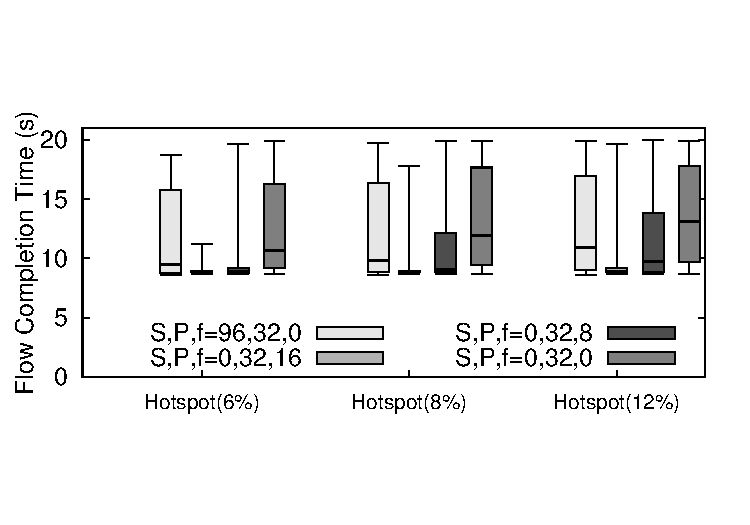
\includegraphics[width=200pt]{zafar_htsim/fct_long_flows_gray.pdf}
} \vspace{-0.7cm} \\
\subfloat[Short-lived flows]
{
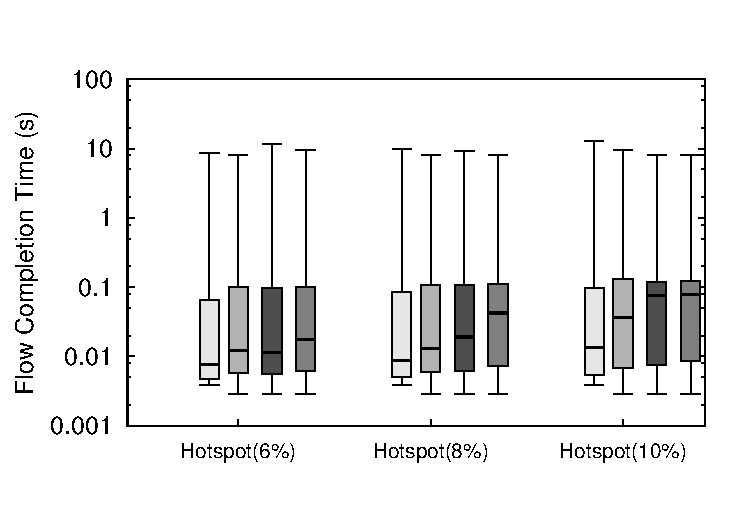
\includegraphics[width=200pt]{zafar_htsim/fct_short_flows_gray.pdf}
}
\caption{A flexible \DC provides similar or better performance relative to overprovisioned networks with much less infrastructure.}
\label{fig:flexibility}
\end{wrapfigure}



To provide the basis for this intuition, we consider an abstract model of a \DC
with $\NumRacks$ \ToR switches  and  $\NumNonToR$ ``core'' switches that
transit traffic between \ToR switches.  Each rack has $\NumMachinesPerRack$
servers and   each  switch (\ToR and core) has $\NumPortsPerToR$ ports. For the
\ToR switches, $\NumMachinesPerRack$ ports connected to the machines, and
$\NumPortsPerToR - \NumMachinesPerRack$ for inter-rack connections.
Furthermore, out of the $\NumPortsPerToR - \NumMachinesPerRack$ inter-rack
ports, suppose $\DegreeFlex$ can be {\em flexibly} rewired. For the non-\ToR
switches, all $\NumPortsPerToR$ ports are connected to other switches.  Now,
for a given $\NumRacks$,  $\NumMachinesPerRack$, and $\NumPortsPerToR$
determined by technology or deployment constraints,  we can define a broad
spectrum of \DC  designs by specifying the 3-tuple $\langle \NumNonToR,
\NumPortsPerToR, \DegreeFlex \rangle$.  For instance, with $\NumPortsPerToR = 2
\times \NumMachinesPerRack$ that is typical of \DC designs today,   $\langle
1.5\NumRacks, 2 \NumMachinesPerRack,  0 \rangle$ corresponds to traditional
{\em static} fat-tree designs and  $\langle 0,  2 \NumMachinesPerRack,
\NumMachinesPerRack \rangle$ captures  an extreme \ArchName point  with no
``core'' switches and full flexibility.  


 Of course, for a given $\langle \NumNonToR, \NumPortsPerToR,\DegreeFlex
\rangle$, we also need to specify the topology created by the ``static'' and
``dynamic'' links.  Rather than explore all possible graph structures for the
{\em static} links, for brevity we only consider {\em random regular graphs}
building on the observation that they provide close-to-optimal
performance~\cite{XXX}.  Thus, we randomly wire the ``static'' links between the
\ToR and  non-\ToR switches.  Based on our preliminary work, we use a greedy
algorithm for the dynamic links where we simply add ``short-cut'' links between
racks with the highest inter-rack demands~\cite{hotnets}.


 Given this abstraction, we evaluate the performance of different \DC designs
by custom extensions to the {\tt htsim} packet-level simulator~\cite{htsim}.
Building on the prior \DC measurements, we consider realistic \DC traffic
workloads~\cite{XXX}, wtih  a baseline {\em uniform} traffic matrix between
racks consisting of short-lived flows with an average size of \plsfill. We
augment this baseline with ``elephant'' or large flows between a subset of
``hotspot'' racks with an average size of \plsfill. In this configuration, {\tt
Hotspot-X} refers to X\% of the rack-pairs having elephant flows. 


 As an illustrative example, we consider the scenario with $\NumRacks$=64 racks
with $\NumPortsPerToR$=32 and $\NumMachinesPerRack$=16 in
Figure~\ref{fig:flexibility} with each link having \plsfill~Gbps.  The result
shows a box-and-whiskers plot with the min, max, and quantiles of the the flow
completion times  for different \DC designs.  Here, $\langle 96,32,0 \rangle$
is a  static regular random graph that provides full-bisection bandwidth with
$\NumNonToR=96$ ``core'' switches.  We consider three  flexible designs with
$\DegreeFlex$ =  0, $\NumPortsPerToR - \NumMachinesPerRack = 16$ (i.e., fully
flexible), and $ \frac{\NumPortsPerToR - \NumMachinesPerRack}{2} = 8$.   The
key takeaway here is that  flexible designs achieve near-optimal or better
performance with significantly less infrastructure requirements.  Specifically,
the $\langle 0,*,* \rangle$ configurations  uses 1.5$\times$ fewer switches and
edges, but achieve  very good performance.  For instance, $\langle
0, 8 \rangle$ configuration increases the  median and 75\%-ile of the flow
completion time for short flows only by  \plsfill and \plsfill respectively but
{\em decreases} that for long flows  by \plsfill and \plsfill respectively. We
have also confirmed that these results qualitatively hold for other  \DC
configurations as well; e.g., with $\NumRacks=$256 racks and
$\NumPortsPerToR$=32 the corresponding improvements are \plsfill.



 %talk about cabling,  power cooling  
\subsection{Case for all-wireless and FSO} 

\myparaq{Why wireless} To realize  a flexible inter-rack fabric, conceptually we need
a reconfigurable ``patch-panel''  between  pairs of racks~\cite{sdnpatch}. Of
course, such a big-switch abstraction is infeasible: (1) it requires very high
fanout ($\NumRacks \times \DegreeFlex$, where $\NumRacks$ is the number of
racks and $\DegreeFlex$ is the number of flexible links at each ToR) and
backplane  switching capacity; and (2)
the  cabling complexity  would be prohibitive and create
operational overheads w.r.t failures, and cooling/airflow
considerations~\cite{XXX}.  For similar reasons, traditional optical
 switching is also not viable.  Finally, this giant switch 
  introduces a single-point of failure~\cite{osa,proteus,helios}. 
 To avoid the need for such a massive switch, 
 we turn to  {\em reconfigurable wireless} links between the  ToR switches.\footnote{Note that we are not proposing a fully wireless data center~\cite{cornell}; our focus is on the ``inter-rack'
fabric.}


%% wireless is not good enough hence fso
\myparaq{Why FSO} The seemingly natural  solution then is 
 traditional radio-frequency (RF) wireless technologies (e.g., 60GHz).
Unfortunately, these  have  many fundamental performance 
limitations: (1)  RF links produce a
large interference footprint due to a wide beamwidth
~\cite{XXX}. \samir{This blames one paper only. This does
not argue why we are discounting every form of RF. Recall the comment from
hotnets reviewer. I can fix this. But the real argument is somewhat involved -- more than a oneliner.}  (2) The beam-steering  technologies
 to implement flexibility are  slow and
inaccurate~\cite{3db} and may additionally increase the interference
footprint~\cite{phased-arrays-rf}; \samir{Need to rephrase, overly sweeping.} 
and (3) The data rates of RF links fall off
rapidly with distance~\cite{3db} and the use 
 of  higher transmit power to increase the range 
 will increse interference and is limited by regulations~\cite{}.
To overcome these limitations, we leverage a somewhat non-standard wireless 
technology---free-space optics (FSO) that uses modulated visible or
infrared (IR) laser beams~\cite{kedar}.\footnote{Unlike traditional optical
links, the laser beam in FSO is not enclosed in a glass fiber, but transmitted
through the air (and hence  ``free space'').}  
 We elaborate on the advantages of FSO vs.\ RF in Section~\ref{sec:fso}.





\subsection{Architecture and Proposed Research}
 
\begin{wrapfigure}{r}{0.4\textwidth}
\label{fig:benefits}
\vspace{-0.6cm}
\centering
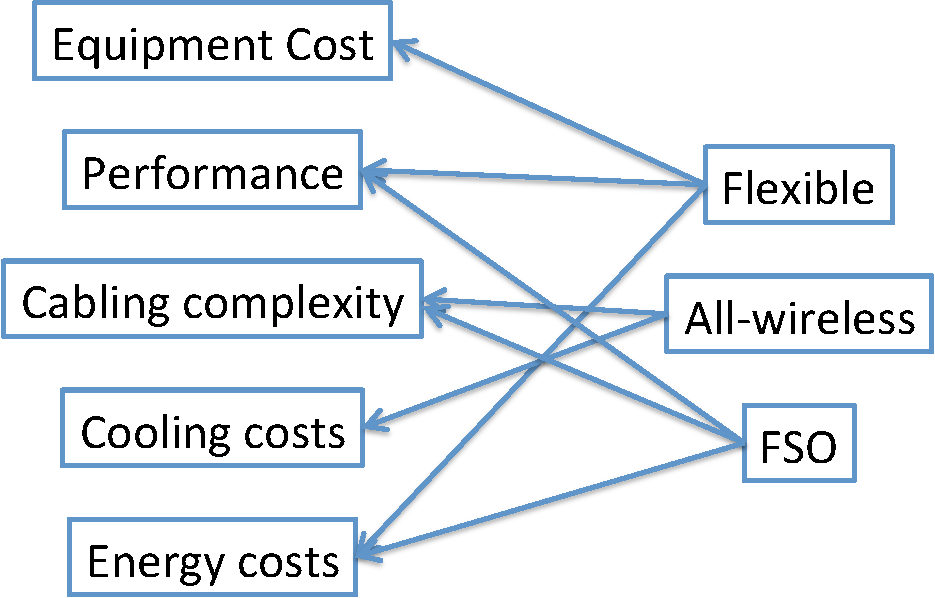
\includegraphics[width=150pt]{PPTFigs/benefitidea.pdf}
\caption{ Key ideas underlying the \ArchName vision and
  how they benefit different 
 of \DC datacenter considerations from Section~\ref{sec:intro}}
\label{fig:benefits}
\vspace{-0.4cm}
\end{wrapfigure}


%% benefits
Combining the above arguments leads us to the architecture   
in Figure~\ref{fig:vision}.  We eliminate the need for a wired backbone network
and rely on a reconfigurable FSO-based wireless fabric.  Each \ToR switch is
equipped with a  pre-specified number of FSO devices and  each FSO device
assembly is capable of precise and fast steering to connect to  target
 FSO devices in other \ToRs. 
  To establish an {\em obstruction-free} optical path, the space
 above the racks is a natural choice for laser propagation as this
 space is roughly free from obstruction~\cite{samirpic}.  The FSO
 transceivers will be anchored on the top of the rack and connected to
 the ToR switch.  \blue{To ensure that the devices themselves do not
   obstruct each other, we propose use of ceiling mirrors as
   in~\cite{3db} (and possibly additional mirrors on the beam path).}

 The \DC management layer  intelligently
reconfigures these devices  to adapt to  changing network requirements.
 Figure~\ref{fig:benefits} summarizes  how the three key aspects of
\ArchName---flexibility, all-wireless, and use of FSOs--- benefit different
considerations of \DC network design: (1) Flexibility  ensures high-performance
with lower cost  and  enables energy reduction~\cite{}; (2) A wireless  fabric
eliminates concerns about cabling complexity and  interference with
cooling~\cite{hpcabling}; and (3) Using FSOs eliminate performance concerns for
a wireless network that might arise from range and  interference constraints. 

While \ArchName is not the first architecture to explore a {\em flexible} \DC
architecture, we highlight  two key aspects of  that make it significantly
different from  prior work on optical or wireless augmentation. First, we are
eliminating the need for a wired core and core switches.  Second,  the use of
FSO-based inter-rack links provides a better alternative to existing RF
wireless or  optical solutions.



%% roadmap
\subsection{Preliminary work:  Cost vs.\ performance tradeoff}

\begin{wraptable}{r}{0.4\linewidth}
\vspace{-0.8cm}
\begin{footnotesize}
\begin{center}
\begin{tabular}{c|c|l}
Architecture & Cost (\$) &  Per-server \\ & & throughput \\   \hline % \hline
 \ArchName (16) & 18.1M  & 1.7 Gbps\\    
3D Beamforming~\cite{} & 17.1M  & 1.1 Gbps\\
Jellyfish~\cite{} 1Gbps & 13M & 1 Gbps\\
Jellyfish 2 Gbps & 26M  & 2 Gbps \\ 
 \ArchName (48) & 37.8M  & 8.5 Gbps \\ 
Fattree/Jellyfish 10Gbps & 57M  & 10 Gbps
\end{tabular}
\end{center}
\end{footnotesize}
\vspace{-0.4cm}
\caption{Cost and performance of \ArchName vs.\ state-of-art proposals for a 512 rack, 48 machines/rack 
 \DC}
\vspace{-0.2cm}
\label{table:cost}
\end{wraptable}

In a preliminary position paper~\cite{hotnets}, we analyzed the
cost-performance tradeoff of candidate \DC architectures for a 512 rack \DC with 48 machines/rack,
  based on publicly available cost projections. Specifically, we consider  full-bisection bandwidth
networks such as FatTree~\cite{XXX} and Jellyfish~\cite{XXX} and the
3D-Beamforming architecture using 60Ghz wireless and ceiling
mirrors~\cite{XXX}.\footnote{We don't consider the all-wireless architecture
of~\cite{cornell} because  it has worse cost-performance tradeoffs; e.g., for
24k machines it costs $\approx 50M$ but only achieves 300-400 Mbps
per-server~\cite{cornell}.} FatTree/Jellyfish-Y Gbps 
 refers to a network with bisection bandwidth  of Y~Gbps, with Y=1,2, and 10.
Here, \ArchName($X$) refers to a hypothetical realization of the \ArchName
vision with $X$ FSO devices on each \ToR switch. 

 We assume that a 64-port 10Gb \ToR switch costs
\$27K: \$11K for the bare switch~\cite{64switch}, and \$16K for 64 10Gbps
optical transceivers at \$250 each~\cite{sfp}. We assume that a 48-port 1Gb
switch costs \$5000~\cite{48-switch-cost}, and each 60GHz radio costs \$1000.
We assume a hypothetical steerable FSO device can be constructed with a total
cost of roughly \$750 (see Section~\ref{sec:fso}).   We conservatively ignore
cabling costs for the wired core for FatTree, Jellyfish, and 3D-Beamforming.
Given the above assumptions, Table~\ref{table:cost} summarizes the cost and the
throughput that different \DC architectures offer based on our simulations.
 The result  shows that   \ArchName offers good cost-performance tradeoffs  w.r.t.\ state-of-art
solutions; e.g., close to 9~Gbps bisection bandwidth at much less cost
compared to a Fat-tree, and 90\% of the performance for 2~Gbps fat-tree at
70\% of the cost.


With this context,  we discuss the three broad research thrusts we need to
address to turn the benefits (Figure~\ref{fig:flexibility},\ref{fig:benefits})
into reality: (1) {\em feasibility of FSOs for \ArchName
(Section~\ref{sec:fso})},   (2) {\em foundations of flexible topology design
(Section~\ref{sec:topology})}, and  (3) {\em effective datacenter management
(Section~\ref{sec:system}).}



\newpage  
\section{Designing FSO Links for Flexible Inter-Rack Networking}
\label{sec:fso}

In this section, we begin by specifying the design requirements for
FSOs and highlight why existing FSO technologies fail to meet the
requirements that the \ArchName vision imposes.  Then, we highlight a
design roadmap for meeting these requirements.

\subsection{Overview and Requirements}

The design of FSO transceivers in \ArchName must simultaneously meet
the following requirements:

\begin{packeditemize}
\item {\em Size, power, and cost effectiveness:} Our goal is to design
  a single FSO transceiver assembly (i.e., including alignment and
  beam redirection machinery) will have $\approx$ 3"x8" footprint so
  that a few tens of such devices can be packed on the ToR.  The power
  consumption should be modest and they must be cost-competitive to
  existing networks.

\item {\em Ability to provide 10-100Gbps data rate:} As DC traffic
  rates are growing~\cite{ananta} and demands for 40~Gbps networks
  emerge, our design must be capable of providing high throughput.

\item {\em Fast and precise alignment and steering :} For FSO links to
  provide high throughput, the transmit/receive devices must be
  precisely aligned. Thus, we need mechanisms for robust re-aligment
  in the presence of environmental effects; e.g., vibrations, changes
  in airflow. Furthermore, to provide fine-grained reconfigurability,
  we need to be able to steer the laser beams to connect to another
  FSO transceiver on another rack determined by the management layer
  in Section~\ref{}.
\end{packeditemize}

% existing solutions suck
Unfortunately, existing FSO transceivers target {\em fixed}
terrestrial long distance (miles) communication~\cite{} and do not
meet our size, power or cost goals.  For example, a typical commercial
system~\cite{lightpointe} is 2 cubic feet, costs \$5-10K for a single
link, consumes \plsfill watts. The reason for the significantly large
numbers is that they have to overcome outdoor challenges --- beam path
variations due to a host of environmental factors~\cite{}, larger
transmit power requirements for longer distances; alignment problems
due to structural swaying etc.  While these issues largely disappear
in the context of DCs and thus create a pathway for size, power, and
cost-optimized design, we have a new requirement of fast
reconfiguration.

%% challenges and approches plan.
We outline the challenges and proposed approaches for FSO design in
\ArchName in a two-step process: (1) Designing the basic FSO link for
a DC-scale operation, and (2) Fast and precise beam redirection to
enable reconfiguration.  Our research here will inform the parameters
(e.g., range, size, \red{cost}) which will be input to the topology
design problems in Section~\ref{sec:topology}.

\subsection{Cost-effective,  Small-Form Factor, and High Throughput FSO Links}

\begin{task}
We will design the FSO link including transmitter, receiver, the
optical beam path, and robust mechanism for correcting misalignments,
while satisfying the the size, power, \red{cost}, and throughput
requirements. We will investigate the size and cost vs.\ performance
tradeoff in a DC-specific context.
\end{task}

\smallskip

%% basic idea -- SFP to FSO, why? Challenges therein.
\para{Converting Optical SFPs to FSOs.}  An FSO communication link has
three basic components: (i) a modulated laser source (typically
infrared) as a transmitter (TX); (ii) a high-speed optical
detector/demodulator receiver (RX); and (iii) a robust optical path
between TX and RX.
%
To demonstrate feasibility of a cost-effective and small FSO link, we
would build an FSO link using the commodity optical SFP (small
form-factor pluggable) transceivers~\cite{}. Optical SFPs are widely
used to interface optical fibers with (electrical) packet switches.
They are small (\plsfill). FSOs based on optical SFPs would easily
satisfy our datarate requirements, and would not create an additional
power burden since SFPs are likely to be used for high datarate links
in DCs anyway.
%
The key difference between optical SFPs and FSOs is that in SFPs, the
laser beam is launched directly into the fiber, while in FSOs, the
laser beam would be launched into free space.
%
The main challenges that arise in converting an SFP into an FSO link
are (i) minimizing beam divergence, and (ii) need for precise
alignment between the TX and RX. We discuss these below.

\para{(i) Divergence.}  A fundamental optical property (unrelated to use
of SFPs) is that the laser beam always {\em diverges} in a cone as it
propagates in free space and accordingly the power density on the
transverse plane goes down with distance. To minimize this divergence,
we need to design suitable {\em collimation lens solutions} on the
optical path near the TX that makes the laser beams roughly parallel
(diverging very slowly with an angle in order of milli-radians, say).
A similar lens near the RX will focus the beam back onto the detector.
While the problem of divergence has been addressed
before~\cite{mustafa2013reintroducing} even in the context of
conversion of optical SFPs to FSO communication, the context of DCs
brings in new design challenges. We articular them below.

From basic optics, an inverse relationship exists between the diameter
of the beam ``waist'' (the narrowest part of the beam near TX) and the
rate at which it diverges beyond the waist. Thus, to keep this
divergence minimal, the beam waist's diameter must be large, which
requires a (larger) lens with a longer focal length and hence, placed
at a larger distance from the SFP. This increases the assembly size --
a concertn for \ArchName. A smaller beam will reduce the assembly
size, but the high divergence may result in the power density at the
RX's detector falling below the ``detection threshold,'' especially
for longer links.
%
Thus, there is a need for careful balance in the design.  
%
Our initial calculations (details ommited, due to lack of space) show
that achieving this balance is indeed possible as the optical SFPs
used for long distance fiber communications have a low detection
threshold. Plus, we can accommodate a long optical path between the
SFP and the lens within a small space by reflecting it multiple times
with small mirrors (as done in~Figure~\ref{fig:optics-layout}).

\para{(ii) Alignment.}  Alignment presents a somewhat related, but critical
challenge. In particular, we want our FSO link design to be tolerant
of small natural shifts of the optical path during regular operation
(e.g., due to rack vibrations or optical drifts due to temperature
variations). This again calls for a larger diameter waist, since a
small diameter may result in insufficient received power if the RX is
off center\footnote{In the transverse plane, the beam power falls off
  from the beam center following a Gaussian profile~\cite{}.} Thus,
we are faced with the same challenges as discussed before.

Regardless of the above, the beam must be re-aligned occasionally to
correct for unexpected shifts and also at the time of
pre-configuration (described momentarily). \blue{We propose to use
  piezoelectric positioners or thermally expandable materials to
  provide fine-grained adjustment to re-align the RX detector at the
  ``peak'' energy position. Commodity technologies are available to
  develop these solutions~\cite{}.}
%%http://www.pi.ws/products/nanopositioning.htm
%
The feedback needed for the correction can be obtained from the DOM
(digital optical monitoring) support available in the optical SFP
standard and carried on the I2C bus via the connectors on the
SFP~\cite {}.\footnote{We suspect for most effects, corrections on the
  RX side are sufficient.  If TX side needs to be adjusted as well,
  the RF-based control channel from Section~\ref{sec:evalplan} can be
  used to coordinate the alignment on both ends.}

\begin{figure}
%\begin{wrapfigure}{r}{0.8\textwidth}
\vspace{-0.5cm}
\centering
\subfloat[FSO prototype on an optical bench set up]
{
%\vspace{-0.8in}
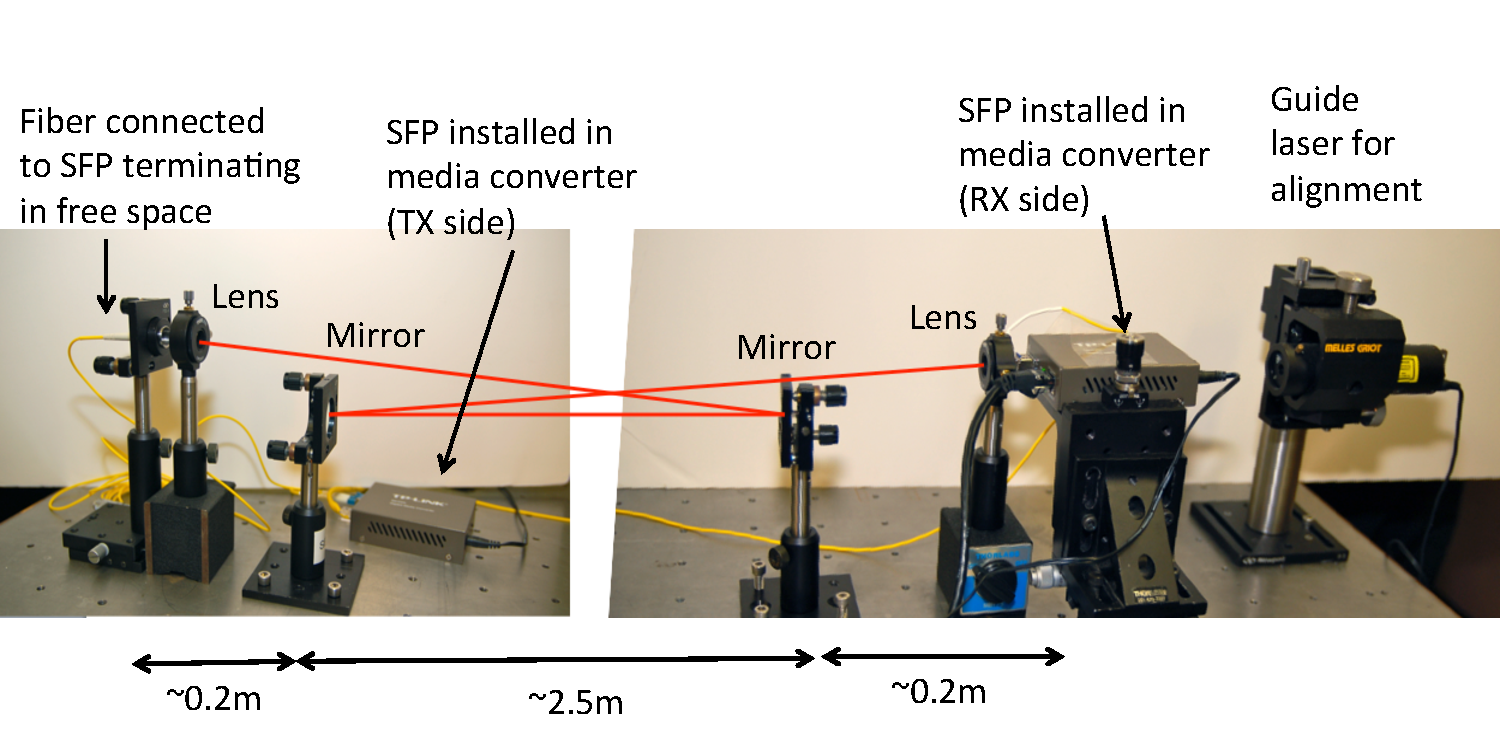
\includegraphics[width=250pt]{PPTFigs/complete-optical-setup-fig.pdf} 
%\vspace{-0.8in}
} 
\hspace*{0.3in}
\subfloat[Throughput stability]
{
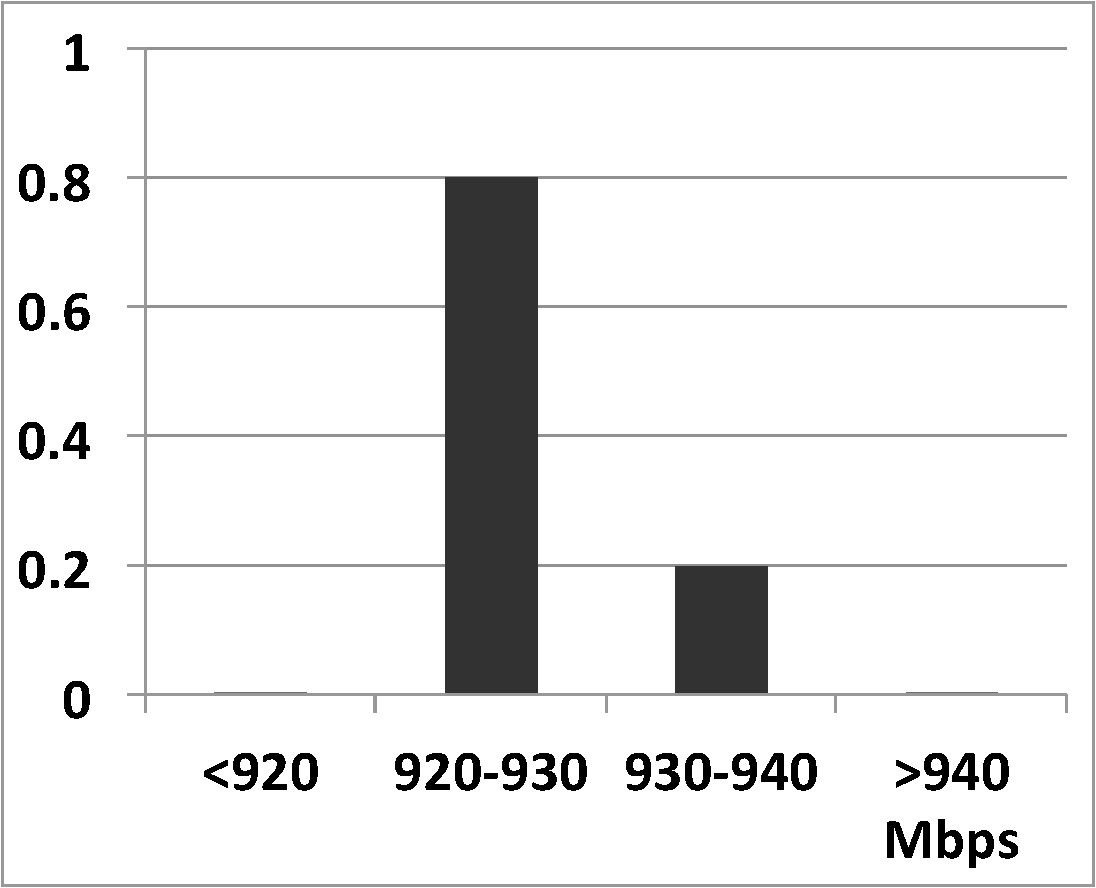
\includegraphics[width=100pt]{Figures/link-thrpt.pdf} 
}
\caption{(a) Experimental prototype showing FSO communication using SFP over ~7.5m.
Note use of mirrors to achieve a long beam path on a standard size optical bench. (The beam is hand drawn.) 
(b) Distribution
of per-second TCP throughputs (in Mbps) over a continuous 30 hour period over ~7.5m.}
\label{fig:optics-layout}
%\end{wrapfigure}
\end{figure}

\para{Preliminary Demonstration of Feasibility.}  We have developed a
proof-of-concept prototype to demonstrate feasibility of designing
FSOs from optical SFPs. See Figure~\ref{fig:optics-layout}. The
prototype uses a pair of 1Gbps SFPs using 1310nm lasers.  We launch
the beam from a single-mode optical fiber connected to the TX SFP on
one end \blue{with the other end terminating in free space.} Due to
the narrow $8-10 \mu\mbox{m}$ fiber diameter, the initial beam
divergence is very large. We used an achromatic doublet lens to
collimate the beam to a roughly 4mm diameter waist with the fiber tip
positioned at the focal point of the lens. (An optical bench and
translating mounts help in the positioning.) The collimated beam
propagates to a distance of 7.5m where an identical lens re-focuses
beam on the RX detector.\footnote{Since the SFP used here uses two
  separate optical paths (for duplex operation), the return link is
  closed using a regular fiber.} We connect the SFPs to a laptop each
via standard media converters~\cite{} and run TCP throughput
experiments for 30 hours to test link stability.
Figure~\ref{fig:optics-layout} demonstrates very stable link
performance comparable to the wired case. We also analyzed the
sensitivitity of our prototype to misalignment between the TX-RX and
found that the throughput is stable up to a transverse shift of
$\pm0.7 mm$.

\subsection{Precise and Fast Beam Redirection}

\begin{task}
\blue{Develop fast and effective beam path redirection techniques to achieve 
reconfiguration in the interconnection fabric.}
\end{task}

\smallskip

% DD, Survey
The result of the previous investigation will provide the basis for a
high-speed reliable link, but we still need a {\em beam steering
  mechanism}.  A wide spectrum of candidate solutions exist for laser
beam steering including phased array techniques~\cite{}. But most of
these are not commodity and some are subjects of active
research. Feasibility and cost-effectiveness for adapting these
solutions for DCs are unknown. For feasibility reasons, we have
investigated two candidate commodity technologies that we will
describe in this section.
% TWO TIMESCALES
Irrespective of the technology used,  there are two fundamental granularities
of  beam ``movements'':

\begin{packedenumerate}
\item{\em Steering:} This refers to the central mechanism where a FSO
  beam emanating from a TX is redirected to a different RX. This must
  be done at a fast time scale -- few millseconds in order to be
  responsive to DC traffic dynamics.  Physical and optical
  limitations, however, induce constraints such that each transceiver
  may only be able to link to only a {\em subset} of other
  transceivers in the DC.  The specific types of constraints may be
  technology-specific as we will see later.

\item {\em Pre-configuration:} Given the above constraint, the above
  subset has to be chosen in a semi-offline fashion for each FSO
  transceiver independently. This gives rise to interesting topology
  design problems that we address in Section~\ref{sec:topology}.
\end{packedenumerate}

%% SCOPE THE WORK
%First we describe the proposed 
%\Preconfiguration can be done simply by using servos that orient 
%specific components to a pre-determineed
%As such, developing a 
%complete solution 
%the \Preconfiguration is outside the scope of the project.

In our proposed research, we will investigate two promising steering
mechanisms, with different tradeoffs as discussed below.

\para{Switchable Mirrors.} Switchable mirrors (SMs) are made from a
special liquid crystal material that can be electrically controlled to
rapidly switch between reflection (mirror) and transparent (glass)
states at millisecond timescales~\cite{sm}. These are used in various
forms of visual aids in niche markets e.g., rear-view video mirror.
Figure~\ref{fig:beam-redirect}(a) conceptually shows how we can use
SMs for beam redirection.  Each FSO device will be equipped with
multiple SMs, with each SM pre-aligned (offline; part of
pre-configuration) to a dedicated beam path. The desired link is
established by swithcing one of the SMs on the TX in the mirror state
and the other SMs in the transparent state. (An analogous arrangement
will be made at the other end, but not shown for ease of
visualization.)  As mentioned earlier, the ceiling mirror redirects
the beam back to the receiving rack, making efficient use of the
above-rack space while minimizing interference. When manufactured at
scale, each small-size SM will have minimal cost ($<$
\$5~\cite{sm-personal}).

\softpara{Preliminary Study.} We evaluated the viability of switchable
mirrors~\cite{hotnets} using a 12" x 15" switchable mirror (SM) from
Kentoptronics~\cite{sm} tuned for the IR spectrum. The switching
latency of the SM is found to be around 250 msec. Because the
switching latency is proportional to the SM’s surface
area~\cite{sm-size}, we estimate a $<5$ msec latency for a small (1" x
1") SM we propose to use. Finally, we confirmed that the FSO beam can
be reflected from conventional mirrors with no loss in TCP throughput
even after multiple reflections.

\begin{figure*}[t] %{r}{0.5\textwidth}
\centering
\subfloat[SM: In the top-half the second SM is in mirror mode,
redirecting the beam to Receiver 1, while the bottom half has SM3 in
 mirror mode and thus redirecting to Receiver 2.]
{
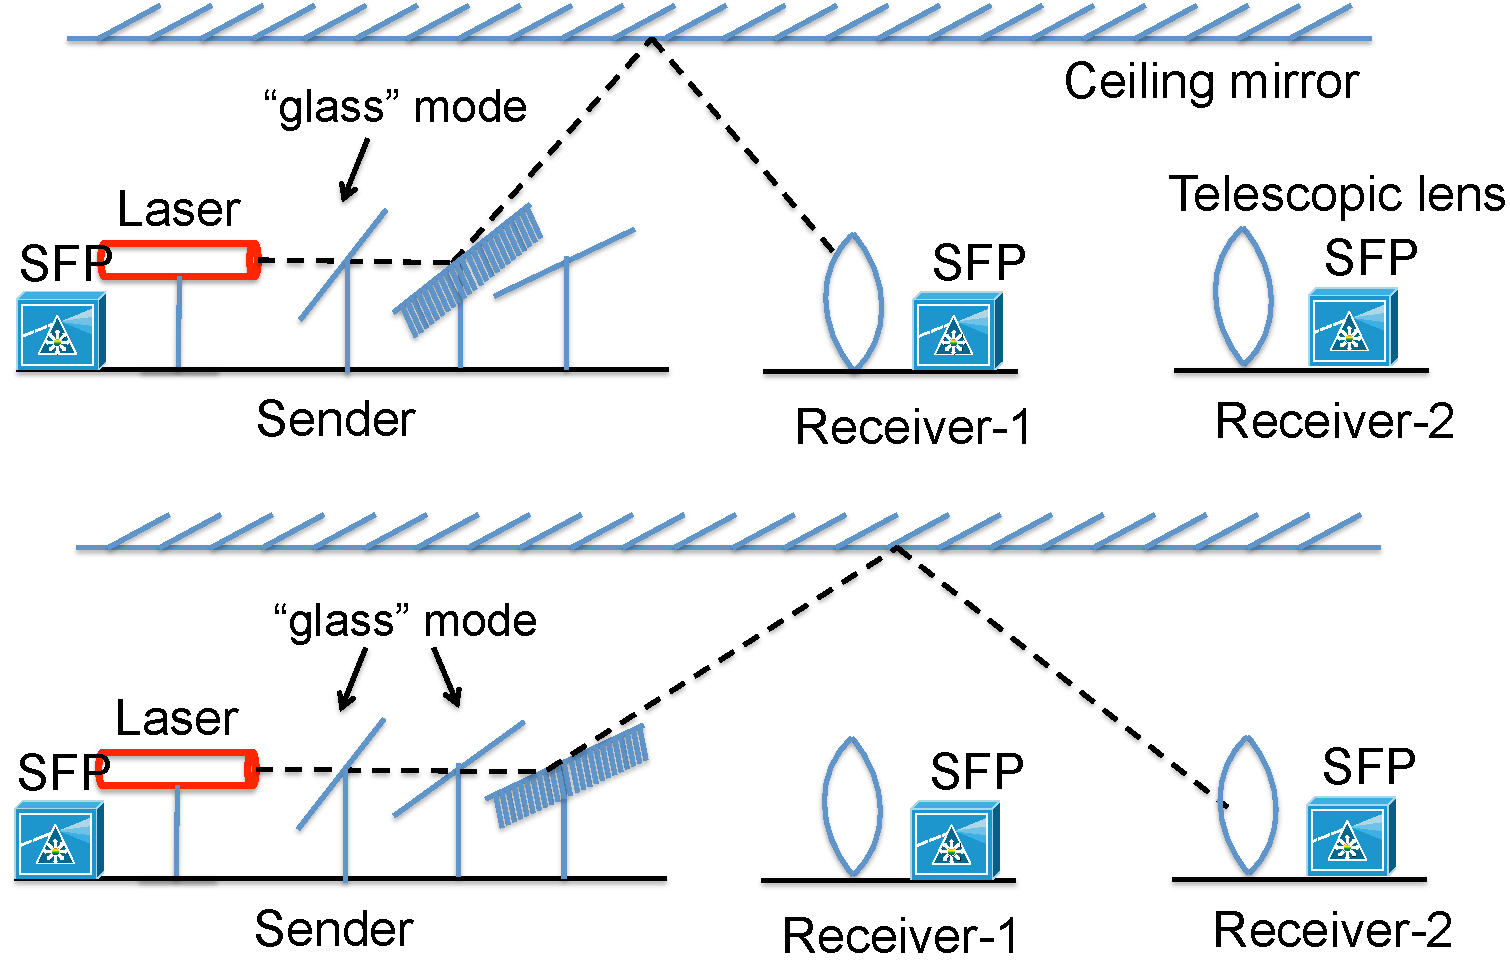
\includegraphics[width=150pt]{Figures/SM-fig.pdf} 
}
\hspace{1cm}
\subfloat[GM: Two mirrors direct incident beam into a rectangular cone. ]
{
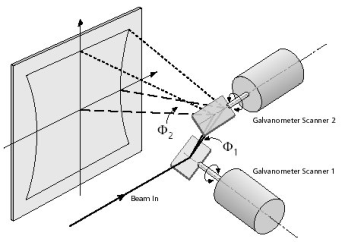
\includegraphics[width=130pt]{Figures/GM-fig.pdf} 
}
\caption{Candidate beam re-direction approaches.}
\label{fig:beam-redirect}
\end{figure*}

\para{Galvo Mirrors.} A Galvo mirror (GMs)~\cite{} is basically a
Galvanometer in principle, except that instead of moving a pointer in
response to current, it moves a small mirror.  GMs are conventionally
used in various laser scanning applications -- both precision
industrial as well as infotainment like laser shows.  As shown in
Figure~\ref{fig:beam-redirect}(b), two computer-controlled, motorized
mirrors are mounted at right angles direct the incident beam into a
rectangular cone.  The (fixed) incident beam can thus be directed into
a rectangular cone under computer control.  Commercially available
systems~\cite{} can provide a cone half angle ($\Phi_1$ and $\Phi_2$)
of $\pm 20^\circ$, for a total rectangular cone angle of $40^\circ$ in
both directions.  A typical pointing accuracy is within 15
$\mu$rad~\cite{}, resulting in a beam positioning precision within
1.5mm for beam paths of up to 100m. Typical steering latency is
\plsfill. \blue{Something about MEMs here.}

\cbl 
\softpara{Custom Building a Small and Inexpensive GM.} Commodity GM
assemblies are expensive (\$ 2000) and much larger than we desire due
to the associated machinary.  One way to minimize the space used on
the rack is to keep only the optical components on the top of rack,
and hide the motor and associated electronics underneath the rack
(using use custom designed extension arms to hold the mirrors) But
additional stability and precision issues must be addressed.  \cb

\para{SM vs.\ GM Tradeoff.}  The key difference between the two
steering mechanisms is the topological possibilites they yield: a GM
can reach {\em any} receiver within the \blue{prescribed} cone (of
limited angle), while use of $\NumSMsPerFSO$ SMs with an FSO provides
$k$ {\em arbitrary} target receivers. Use of GM may obviate the need
for additional alignment (e.g., piezo electric positioners), but
commodity GM assemblies are much larger than we desire due to the
associated machinary. In our research, we will systematically
investigate the impact of these tradeoffs, and use a hybrid
architecture consisting of both steering mechanisms.

\para{Pre-configuration Machinery.} Note that SMs and GMs will need to
be aligned (or oriented), to target the desired set of
receivers. However, this is done in a semi-offline fashion, so speed
is not of the essence. In particular, the desired alignments can be
pre-computed and achieved by servos that simply orient the attached
component (e.g., SM, GM) to the desired position. Micro adjustments
can be done using the piezo-electric positioners described before. We
skip further details of the above pre-configuration machinery since it
is outside the scope of this project. However, we discuss
pre-configured topology design challenges in the next section.

\hg{I removed the ``overall cost'' para; I think its unnecessary, and
  can instead go in {\em budget justification}.}  









\newpage
\section{Pre-Configured Flexible Topology Design}
\label{sec:topology}

The \ArchName hardware, discussed in the previous section, impose  
physical and geometric constraints on the network design.  For
instance, the size of the FSO device assembly limits the number of
FSOs that can be placed on the rack and the cost/range of steering
mechanisms may also come into play. Our goal then is to design the
most cost-effective and efficient flexible network design that can
work within these constraints.

\begin{wrapfigure}{r}{230pt}
\centering
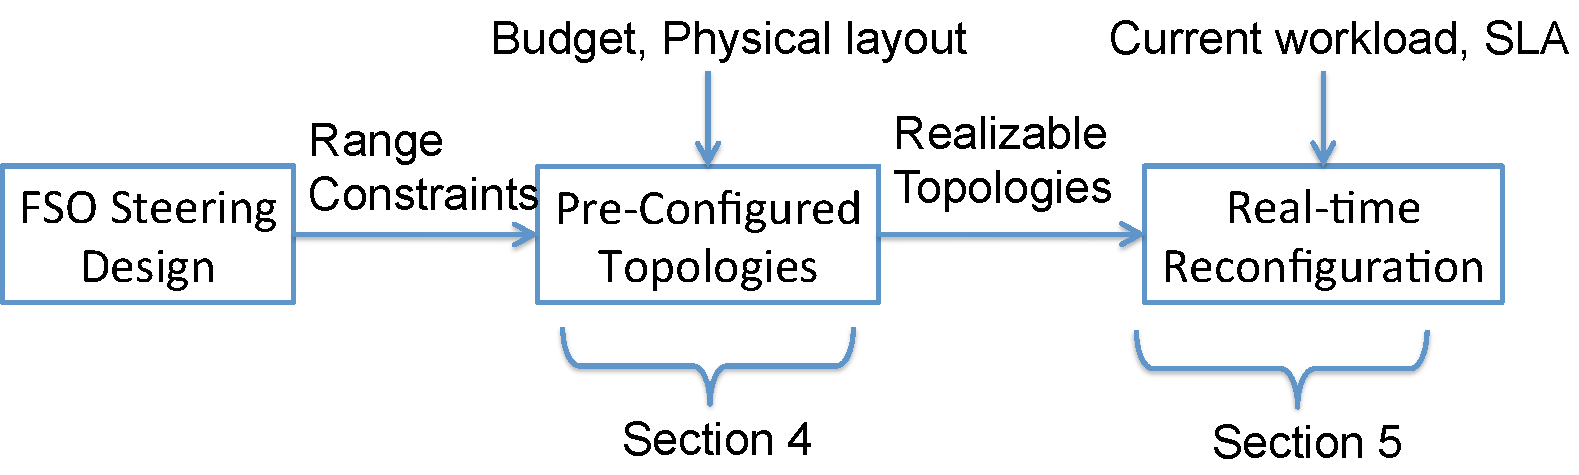
\includegraphics[width=220pt]{PPTFigs/OptimizationInteraction.pdf}
\caption{Interaction between the design constraints induced by FSO
steering choices, the selection of preconfigured topologies, and the
real-time topology selection} 
\label{fig:345}
\end{wrapfigure}

In our context, there are essentially two \blue{stages of network
  design} done at different timescales of operation.
\underline{First}, we need to {\em pre-configure} the network and FSO
assembly; e.g., choosing number of FSOs per rack, the specific
alignments of the different SMs, or \blue{scoping} the beam angle of
the GMs. This needs to be done at coarse time granularity (e.g.,
monthly), because of the time incurred in changing such a
pre-configuration setup. \underline{Second}, given this pre-configured
setup, we need to choose a {\em runtime} topology by activating a
subset of links, at finer timescales (i.e., few millseconds) based on
the prevailing traffic load. Thus, we envision the design workflow in
  Figure~\ref{fig:345}.  In this section, we focus on the first
  network design problem done at a coarser timescale, viz., the
  pre-configuration problem.  We defer the runtime operation (called
  {\em reconfiguration}) to Section~\ref{sec:reconfig}.

\green{Essentially, the pre-configuration problem is: Given an overall
  budget and phyiscal constraints, determine a range of network
  parameters---number of machines per rack, number of FSOs per rack,
  number of FSOs equipped with GM vs.\ SM, number of SMs per FSO, the
  pre-orientation of GMs, and the pre-alignment of SMs---that can
  deliver good performance.}
%
This problem is significantly different from prior theoretical work in
network design~\cite{} on two fronts: (1) {\em flexibility} requires
us to rethink topology design algorithms and traditional performance
metrics, and (2) the \ArchName hardware elements impose unique
physical, budget, and geometric constraints. Thus, we break down our
proposed research into two stages.  First, to \blue{understand the
  theoretical implications of topology flexibility}, we focus on a
more abstract problem of designing an optimal ``pre-configured
flexible topology'' (\PCFT). Then in Section~\ref{sec:bbo}, we use
these insights to revisit the budget-based \ArchName network design
problem.

\subsection{Foundations of Pre-Configured Flexible Topology Design (\PCFT)} 
\label{sec:pcft}

\begin{wrapfigure}{r}{160pt}
\vspace{-0.2in}
\centering
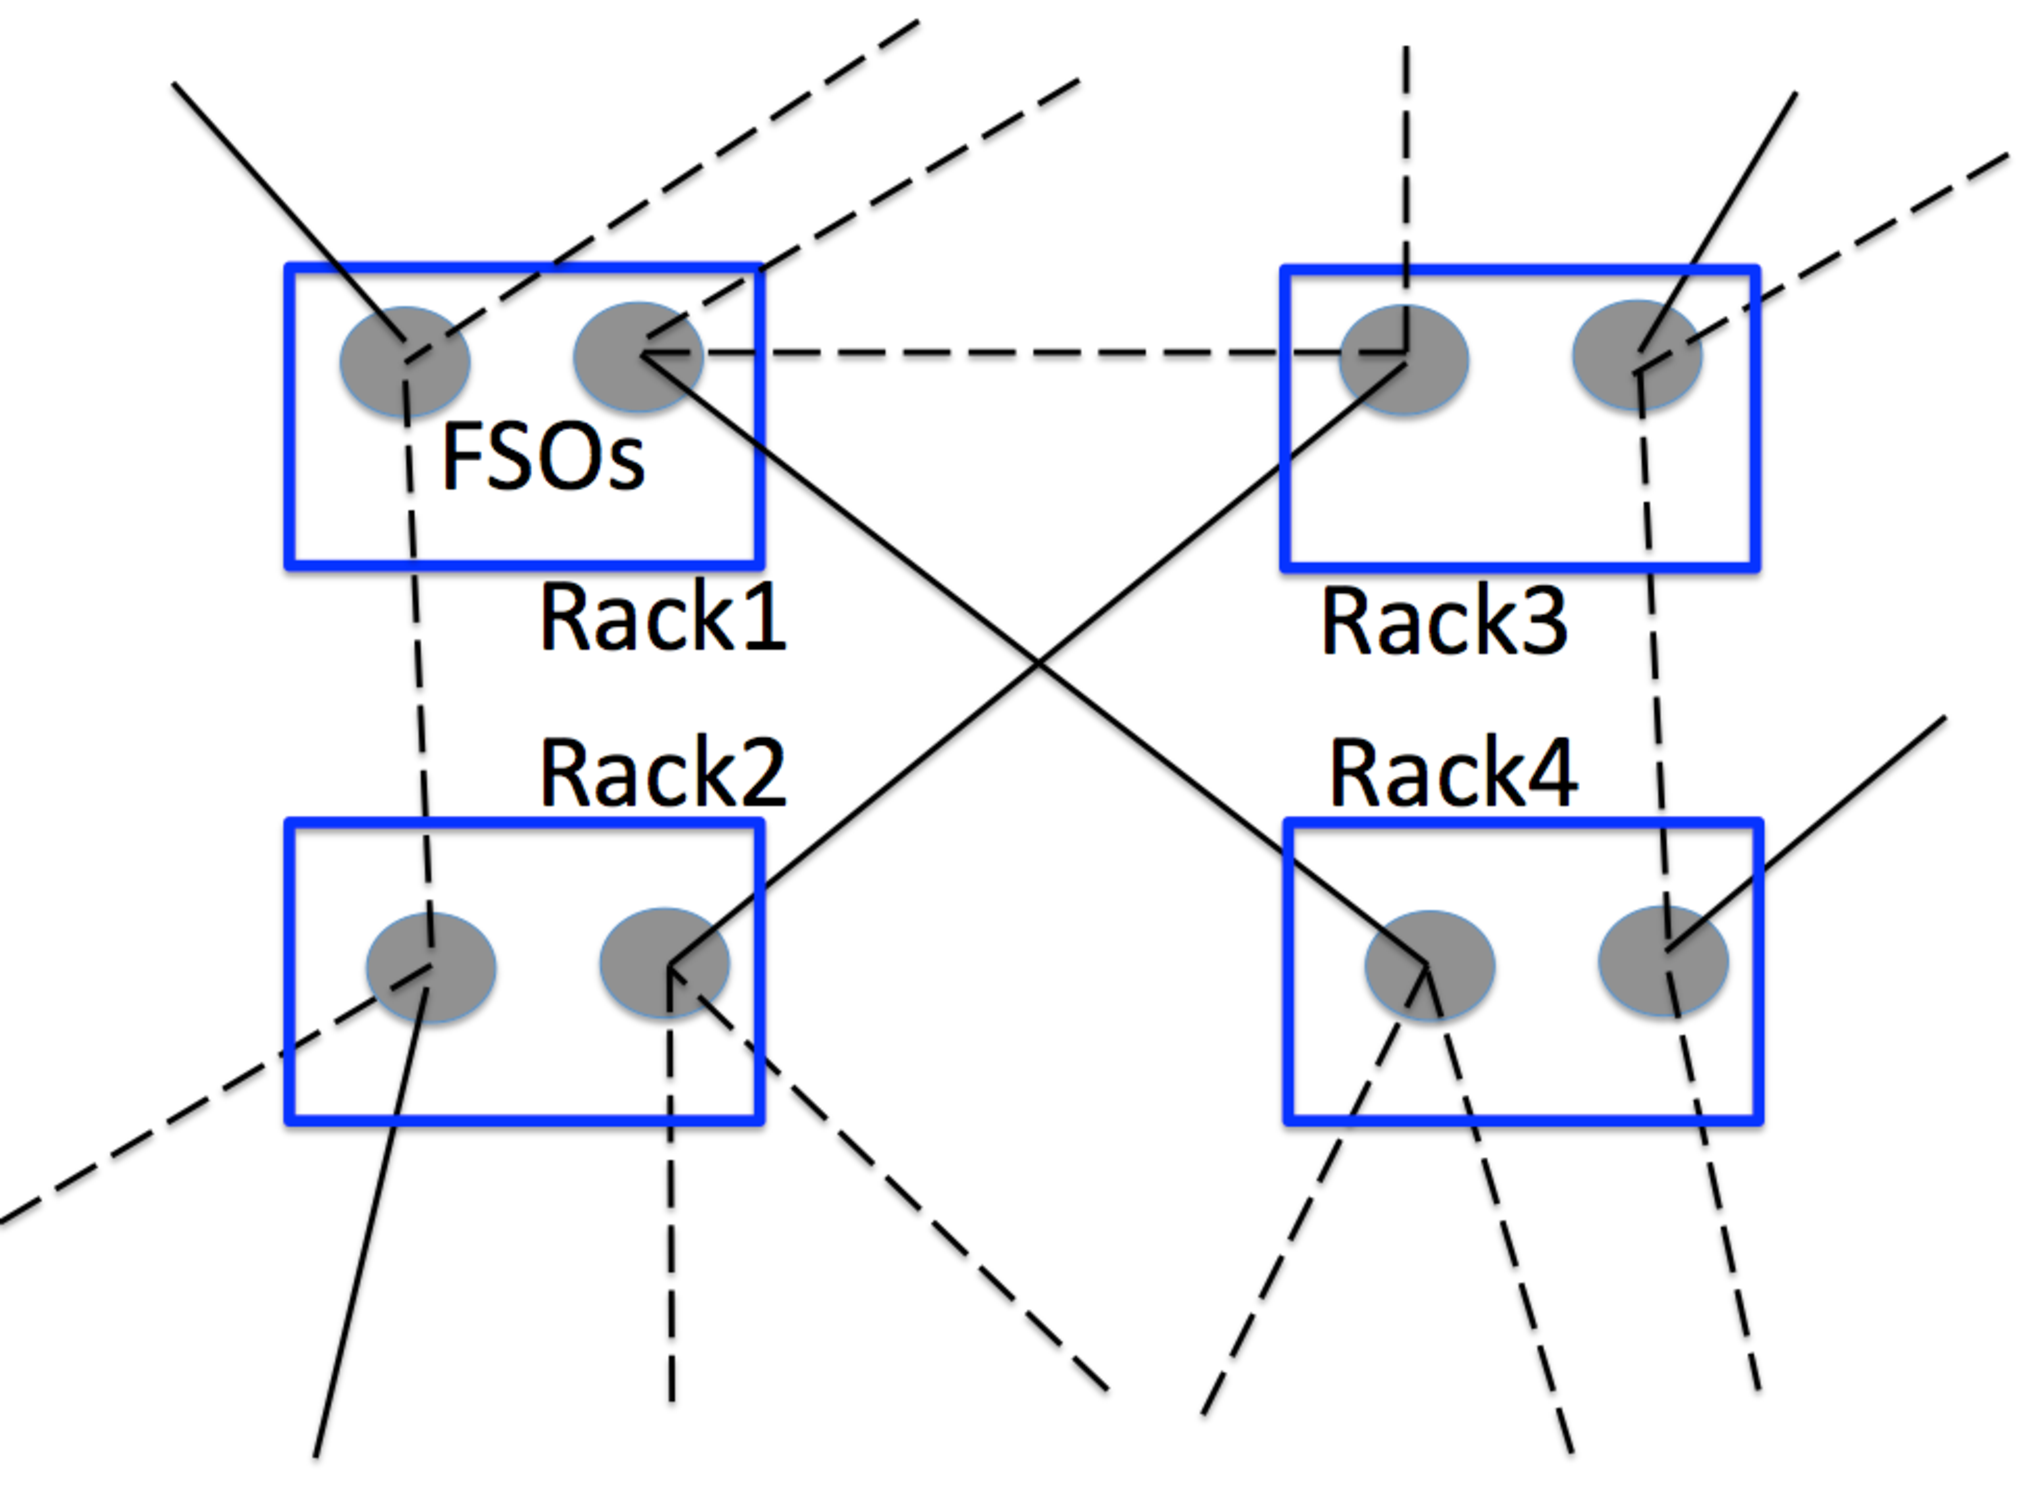
\includegraphics[width=160pt]{PPTFigs/pcft.pdf}
\vspace*{-0.4in}
\caption{A pre-configured flexible topology (PCTF) with candidate
  links (solid and dashed). Number of FSOs per rack ($m$) is 2, and
  the number of candidate links per FSO ($\FSODegree$) is 3. The set
  of solid (active) represents one possible realizable topology.}
\label{fig:pcft}
\end{wrapfigure}

To gain insights into the theoretical foundations of the problem, we
abstract away the details of the SM or GM or the cost budget and focus
on the following problem: Given the number of racks $\NumRacks$,
number of FSOs $\NumFSOs$ on each rack, and the maximum number of {\em
  candidate links} $\FSODegree$ per FSO \blue{that each FSO can be
  steered to}, the {\em pre-configured flexible topology (\PCFT)
  design problem} is to determine the set of links connecting pairs of
FSOs, so as to optimize the ``dynamic bisection bandwidth'' of the
network (defined below).

\softpara{Terminology.} A \PCFT essentially is a $k$-regular graph
over the $m$ FSOs, where each edge is called a {\em candidate link}
and represents an achievable communication link. However, at any point
during runtime, only one candidate link per FSO can be {\em active};
thus, the set of active links form a matching over the FSOs. Given a
\PCFT, any matching over the FSOs is called a {\em realizable
  topology} of the given \PCFT. See Figure~\ref{fig:pcft}.
%
\green{Thus, the PCFT problem can be thought of as constructing a
$\FSODegree$-regular graph over $\NumRacks\NumFSOs$-nodes such that
the {\em set} of matchings (i.e., realizable topologies) of the graph
maximizes the dynamic bisection bandwidth (defined next).}

\begin{task}
\label{task:pcft}
We will investigate the theoretical foundations of flexible topology
design that maximizes dynamic bisection bandwidth in conjunction with
other measures of network goodness (e.g., diameter).
\end{task}

\mypara{Rethinking Metrics for Flexible Topologies} The traditional
bisection bandwidth metric~\cite{} reflects a {\em static} perspective
of the topology. However, in our context, we should instead consider
the notion of {\em dynamic} bisection bandwidth (DBW) since different
realizable topologies can be used for different communication
requirements. Formally, the dynamic bisection bandwidth of a given
pre-configured topology $\Pi$ can be defined as follows. Let $T$ be
the set of realizable topologies of a given pre-configured topology
$\Pi$, $P$ be the set of partitions of the given network into two
equi-sized sets of machines, and $BW(t,p)$ be the bandwidth of a
(realizable or static) topology $t$ for the partition $p$ (i.e., the
cut-size in $t$ corresponding to $p$). Then, the traditional notion of
bisection bandwidth for a (static) topology $t$ is given by $\min_{p
  \in P} {\rm BW}(t, p).$, while the {\em dynamic bisection bandwidth}
DBW($\Pi$) for the pre-configured topology $\Pi$ is defined as:
$$\min_{p \in P} \max_{t \in T} {\rm BW}(t, p).$$

In addition to just maximizing DBW, we also consider the objective of
maximizing DBW under the constraint of bounded network diameter.
Network diameter is a reasonable way to bound worst-case latency,
which has also been considered as an objective in designing datacenter
topologies~\cite{rewire-20-39}. We also also use an appropriate notion
of {\em dynamic diameter} (as for DBW above) instead of the
traditional notion of network diameter.

\mypara{Connection to Known Graph Problems} In general, the PCFT
problem is in the class of the {\em network design problem
  (NDP)}~\cite{ndp-survey} (and more specifically, {\em
  degree-constrained subgraph} problem), wherein, given a graph, the
goal is to extract a (degree-constrained) subgraph satisfying some
design criteria and optimizing a given objective function.  What
distinguishes the PCFT problem from the prior-addressed NDP problems
is the choice of our objective function, viz., dynamic bisection
bandwidth.

The special case of the PCFT problem, when $\FSODegree=1$, actually
boils down to constructing an $\NumFSOs$-regular graph over
$\NumRacks$ nodes with maximum (static) bisection bandwidth. The
closest known problems to this $\FSODegree=1$ case of our PCFT problem
are: (a) Computing the bisection bandwidth of a given \blue{regular}
graph; this problem is known to be
NP-hard~\cite{bui-leighton-comb-1987}, with the best known
approximation-factor of $O((\log n)^2)$~\cite{fiege-focs-2000}. Our
PCFT problem is very different from this problem. (b) Determining an
upper-bound on the bisection bandwidth of $\NumFSOs$-regular graphs of
size $\NumRacks$, for a given $\NumFSOs$ and $\NumRacks$; this problem
has been addressed extensively, and non-tight upper-bounds (have been
determined for small values (upto 4) of
$\NumFSOs$~\cite{monien-2006}. Note that this upper-bound problem can
actually be reduced to the $\FSODegree=1$ version of our PCFT
problem. {\it The above results suggest that the PCFT problem is very
  likely intractable, even for $\FSODegree=1$.}


\mypara{Proposed Approaches} We will pursue three different approaches
for the PCFT problem. The first approach builds upon designs with high
static bisection bandwidth, the second approach builds upon solutions
to special cases of the dual-problem, while the third is a heuristic-based
approach.

\begin{packeditemize}
\item {\em Static to Dynamic Conversion.} One reasonable approach to
  solve the PCFT problem would be to start with constructing a
  $\NumFSOs\FSODegree$-regular graph of $\NumRacks$ nodes with a high
  (static) bisection bandwidth, and then group the
  $\NumFSOs\FSODegree$ candidate links at each node into $\NumFSOs$
  sets of $\FSODegree$ links each so as to maximize the dynamic
  bisection bandwidth. For the \underline{first step}, there are only
  a few results on explicit construction of general graph classes with
  high bisection bandwidth~\cite{peres}. In particular, $d$-regular
  Ramanujan Graphs~\cite{rewire-18} of are known to have a bisection
  width of at least $((d/2 - \sqrt(d-1))n/2$, but their construction
  is mostly algebraic. Other graph classes of interest are Cage
  graphs~\cite{cage}, which have a large \blue{girth} (length of
  smallest cycle). In our specific context of small values (a few
  hundreds) of $\FSODegree\NumFSOs$ and $\NumRacks$, we can
  investigate bisection bandwidth of certain classes of regular
  graphs, and pick ones that suggest a high bisection bandwidth
  \blue{with low diameter}; in particular, due to symmetry of
  nodes/racks, we can also restrict ourselves to ``symmetric'' regular
  graph such as distance-transitive graphs. For the \underline{second
    step} of grouping candidate links, we will employ certain
  heuristics. E.g., we can number the $\NumRacks$ nodes from 1 to
  $\NumRacks$ and group the $\NumFSOs\FSODegree$ links into $\NumFSOs$
  sets based on the ranges of node numbers they connect to. Such a
  heuristic will guarantee a ``uniform'' division of links into sets
  across the nodes.

\item {\em Dual-based Approach.}  If each rack contains
  $\NumMachinesPerRack$ machines and the links (between a machine and
  the ToR switch, or a pair of FSOs) have a unit bandwidth, then the
  optimal desired bisection bandwidth is
  $\NumRacks\NumMachinesPerRack/2$. We note that, for uniform link
  bandwidths, the inter-rack and inter-machine bisection bandwidths
  are same. Now, let us consider what values of $\FSODegree$ and
  $\NumFSOs$ can enable this DBW value of
  $\NumRacks\NumMachinesPerRack/2$. We consider two extremes: (a) If
  $\FSODegree=1$, then it can be shown that \blue{$\NumFSOs =
    \min(\NumRacks/2+\NumMachinesPerRack, 7\NumMachinesPerRack)$
    suffices\footnote{By using $7l$ ports on a ToR switch, we can
      simulate a Fat tree architecture.} (but not necessarily
    optimal).} For large values of $\NumRacks$ and
  $\NumMachinesPerRack$, it is known~\cite{book-28-29} that
  $\NumFSOs=2\NumMachinesPerRack$ would almost always work. (b) If
  $\FSODegree$ can be an arbitrarily high, then the optimal value of
  $\NumFSOs$ required is $\NumMachinesPerRack$ (for $\FSODegree=n/2$);
  here, for $\NumFSOs=l$, the $\FSODegree$ required (=$\NumRacks/2$)
  is also optimal. The above resuls hold for any DBW value that is an
  integral multiple of $\NumRacks$.
%
The above near-optimal solutions for certain special cases of the
``dual'' problems (i.e., given a desired DBW value, minimize $\NumFSOs$ or
$\FSODegree$ for a given $\NumRacks$ value) gives us some insights into solving the
PCFT and its dual problems.  In particular, if we can solve the above
dual problem of minimizing $\NumFSOs$, given $\FSODegree$, $\NumRacks$, and a desired DBW
value, for arbitrary $\FSODegree$ values and integral of $\NumRacks$ values of DBW,
then it is easy to derive an approximation algorithm for the PCFT
problem that has only an {\em additive} approximation-factor of $\NumRacks$.

\item{\em Simulated Annealing (SA-PCFT).}  Simulated Annealing (SA)
  heuristics~\cite{} have been used with great success for
  optimization problems. \blue{In our context, since the PCFT design
    is done offline, we can afford the convergence time incurred by an
    SA approach.}  To design an SA approach for our PCFT problem, we
  need three key components: \underline{First}, we need good ``seed''
  (starting) solutions; here, we could use one of our earlier
  approaches, or as in~\cite{rewire}, use graphs with a ``large
  spectral gap''~\cite{rewire,spectral,rewire-18} which are known to
  have desirable properties (e.g., low
  diameter~\cite{spectral-diameter}).  \underline{Second}, we need
  ways to generate ``neighboring'' solutions; for this, we can use
  \blue{simple transformations} that transform a regular graph to
  another. E.g., the transformation that changes the edges ${(a,b),
    (c,d)}$ to ${(a,c), (b,d)}$ can be used iteratively to construct
  any regular graph from another.  \underline{Lastly}, we need an
  efficient heuristic for computing DBW (PCTF's objective function) of
  a given graph; for this, we will investigate generalization of the
  following approaches: (i) Well-known efficient heuristics, viz.,
  SA~\cite{} and Kernighan-Lin~\cite{} for computing the bisection
  bandwidth, and (ii) a recent result~\cite{rewire} that uses Valiant
  (or, two-state) load balancing technique~\cite{valiant} to compute a
  {\em lower bound} on the bisection bandwidth.

  The above SA-PCFT approach can also be generalize to maximize an
  appropriately defined {\bf traffic-aware DBW objective}, based on
  coarse statistics available on inter-rack traffic. \green{Note that
    since pre-configuration can only be done on an infrequent basis
    (e.g., weekly), so we are only interested in coarse traffic
    knowledge.}  One simple form of inter-rack traffic statisfics
  could be in the form of a weights between every pair the racks, and
  the DBW definition can be appropriately tailored as
  in~\cite{leighton-99} for multi-commodity min-cut. \blue{In our
    research, we will also consider incoporating more sophisticated
    traffic models~\cite{}.}
\end{packeditemize}

\subsection{Budget-Based Optimization}
\label{sec:bbo}

Formally, given the total number of machines to interconnect, physical
constraints, overall budget, and pricing of relevant hardware devices,
the \BBO problem is to determine the following such that the dynamic
bisection bandwith is maximized: (a) Number of machines
($\NumMachinesPerRack$) per rack and thus, the number of racks
($\NumRacks$), (b) number of FSOs ($\NumFSOs$) per rack and thus, the
number of ports on the ToR switch, (b) Number of FSOs ($\NumFSOsWithGM
\leq \NumFSOs$) that are each equipped with a GM and the number of SMs
($\NumSMsPerFSO$) on each of the remaining $(\NumFSOs -
\NumFSOsWithGM)$ FSOs, on each rack, and (c) the {\em pre-orientation}
of each of the GMs and {\em pre-alignment} of each of the SMs in the
system.

\begin{task}
\label{task:bbo}
We will design efficient algorithms for the Budget-Based Optimization
Problem (\BBO) with the objective of maximizing dynamic bisection bandwidth.
\end{task}

\mypara{Proposed Approach} Based on our insights from the previous
section, we will use the following approaches to address the \BBO
problem:

\begin{packeditemize}
\item
{\em PCFT-Based Algorithm.}  We can use any of the PCFT algorithms as
a subroutine to solve the BBO problem as follows. \underline{First},
we convert the given budget and physical constraints, and the pricing
information into a constraint equation over $\NumRacks$ (number of
racks), $\NumFSOs$ (number of FSOs per rack), and $\FSODegree$ (the
number of candidate links per FSO). \blue{To constrain $\FSODegree$,
  note that $\FSODegree\NumFSOs = c\NumFSOsWithGM + (\NumFSOs -
  \NumFSOsWithGM)\NumSMsPerFSO$, where $c$ is the number of candidate
  links a GM can be steered to use and can be assume to be a
  constant.}
%
\underline{Second}, we solve the PCFT problem for various $\NumRacks$,
$\NumFSOs$ and $\FSODegree$ that satisfy the above budget constraint
for a given $\NumFSOsWithGM~(\leq \NumFSOs$).  Then, we convert each
PCFT solution to a design realizable by $\NumFSOsWithGM$ GMs and
($\NumFSOs - \NumFSOsWithGM$) sets of $\NumSMsPerFSO$ SMs each, on
each rack, and estimate its DBW using one of the approaches described
earlier. \underline{Lastly}, we explore the space of
$\NumRacks,\NumFSOs,\FSODegree, \NumFSOsWithGM$ efficiently using
standard search techniques, to compute an efficient network design for
the given budget and pricing.

\item
{\em Extending SA-PCFT.}  We can modify our Simulated Annealing
approach for the PCFT problem to solve the \BBO problem, by
appropriately modifying the transformation operator to generate
neighbors of a particular network design. Here, the neighbors of a
design may include designs with slightly different values of
parameters $\NumRacks$, $\NumFSOs$, $\FSODegree$, $\NumFSOsWithGM$,
and/or candidate links, under the budget constraints.
\end{packeditemize}

\newpage
\section{\ArchName Network Management}
\label{sec:system}

In this section, we focus on the design of a {\em datacenter
  management layer} that uses building blocks from previous sections,
to implement a \blue{feasible} reconfigurable datacenter network.
%
We start with describing the high-level roles of the different
components of the management layer. See Figure~\ref{fig:mgmt}.

\begin{wrapfigure}{r}{0.5\textwidth}
\vspace{-1cm} 
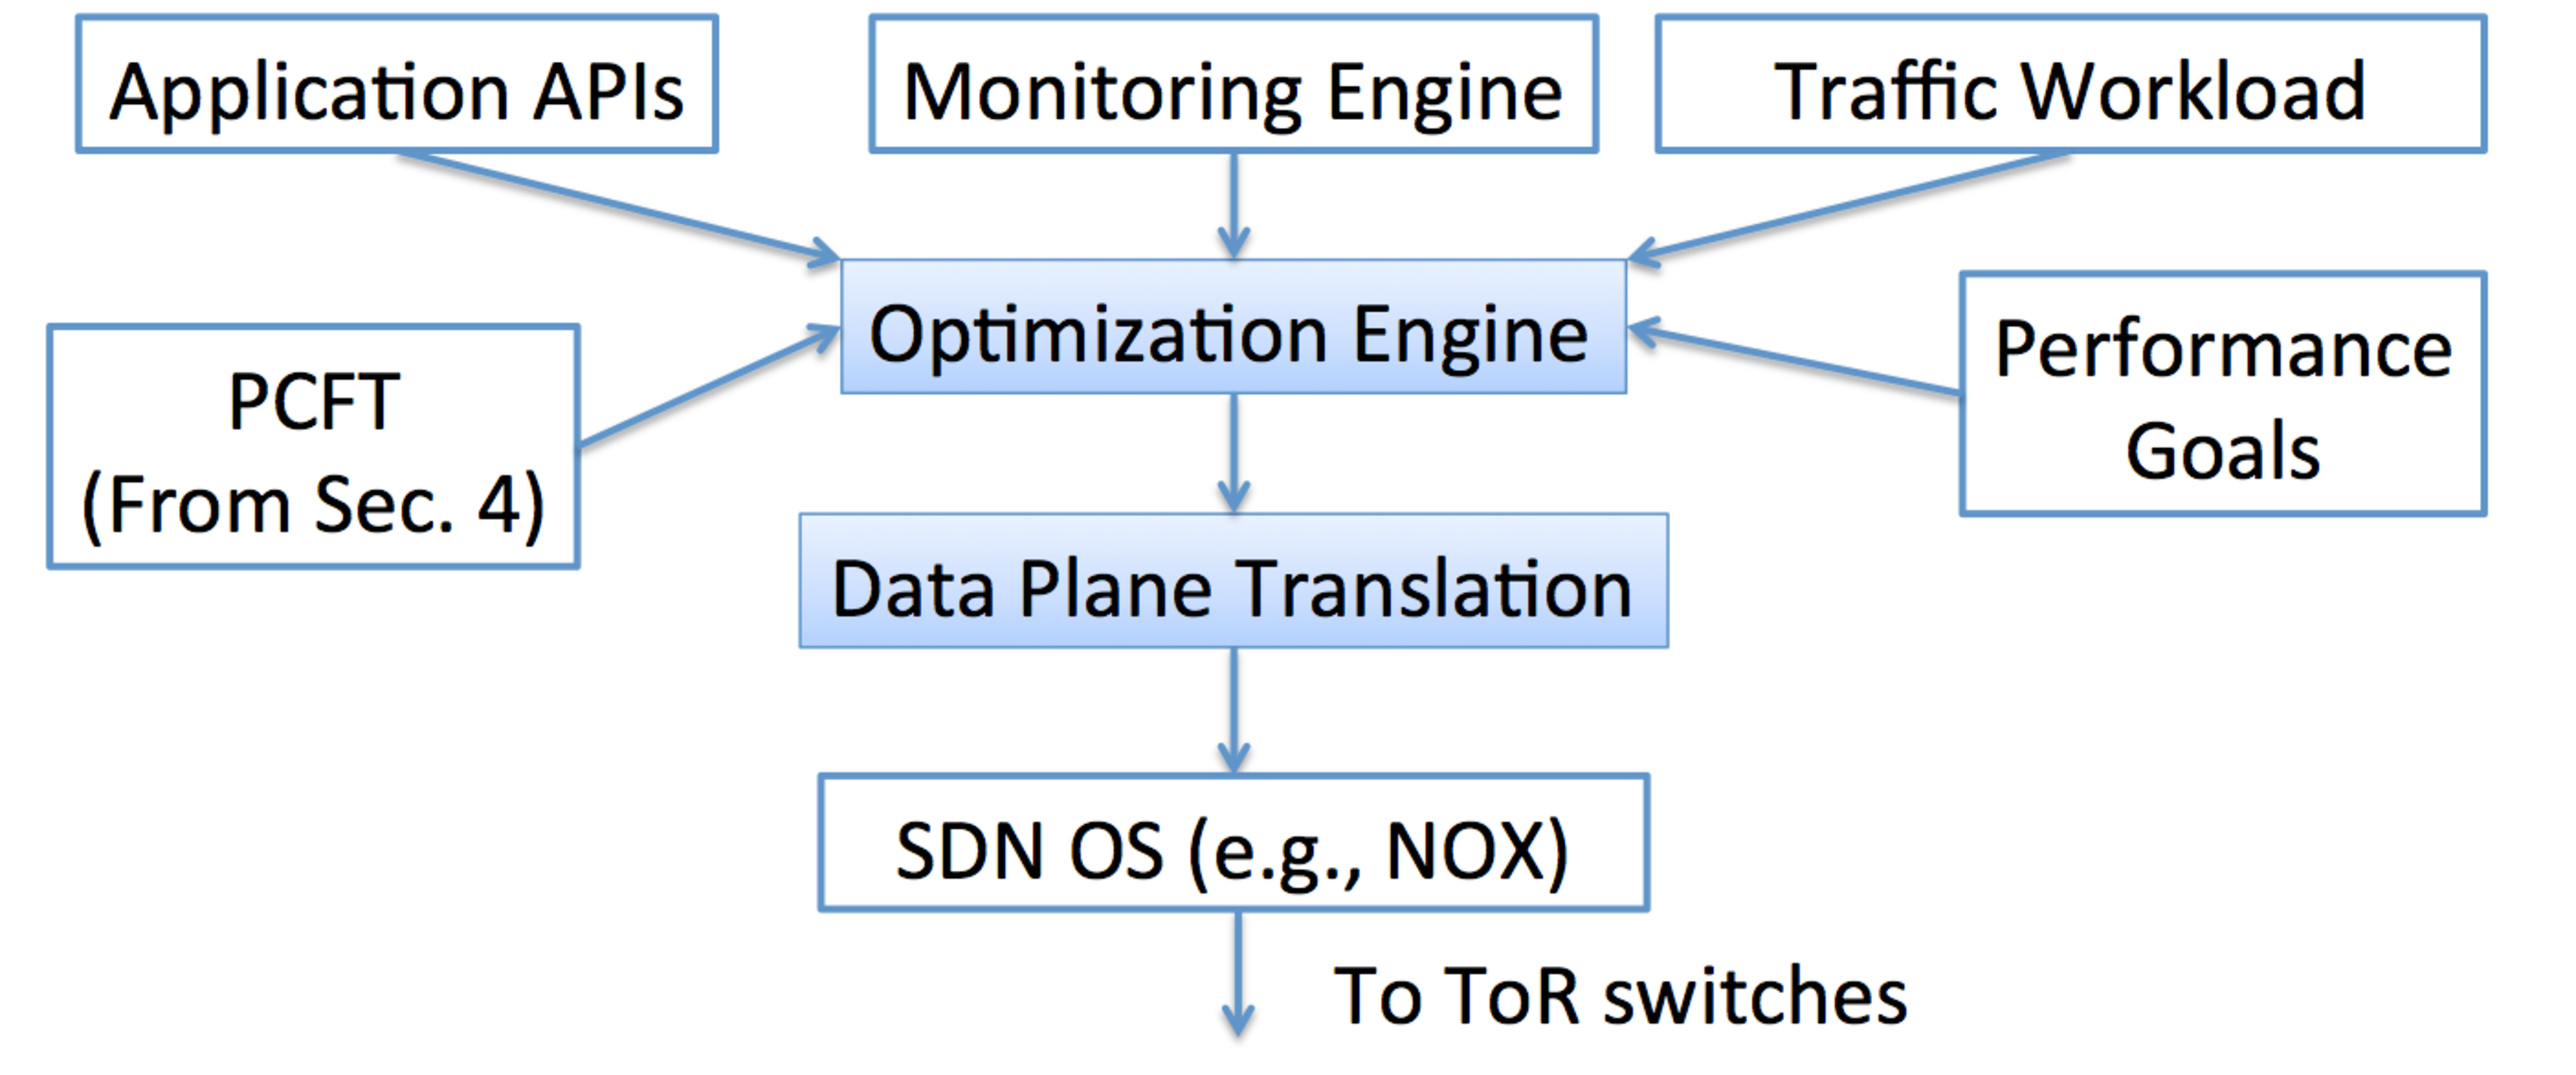
\includegraphics[width=240pt]{PPTFigs/sysoverview-new.pdf}
\vspace{-0.8cm} 
\caption{Overview of the \ArchName management layer}
\vspace{-0.6cm} 
\label{fig:mgmt}
\end{wrapfigure}

\begin{packeditemize}
\item {\bf Monitoring Engine (ME):} ME provides network status
  information (e.g., links status, traffic patterns, or views
of ``elephant'' flows~\cite{hedera,devoflow,conext13ericson})
to the management layer. 

\item {\bf Optimization Engine (OE):} Given the offered traffic
  workload, a pre-configured flexible topology (PCFT), and the current
  network state (e.g., link status), the optimization engine devises
  an efficient {\em reconfiguration and traffic engineering strategy}
  so as to optimize desired performance goals.

\item {\bf Data Plane Translation Engine (DPE):} DPE translates the
  OE output into an efficient data plane strategy.

\item {\bf Application APIs:} APIs enable the users/tenants to inform
    application details (e.g., expected traffic patterns,
    single/multi-path TCP) to the optimization and data plane modules,
    \blue{to best leverage the benefits of \ArchName.}
\end{packeditemize}

\softpara{Plan.} For the ME, we will leverage past work on scalable 
traffic matrix and elephant flow
detection~\cite{hedera,devoflow,yingzhangconext13}.  Similarly, we
will extend prior work on APIs for applications to expose traffic
patterns~\cite{coflow,bigdatahotsdn}.
%
We address OE and DTE in the following subsections. In the last
subsection, we address design of a wireless out-of-band control
network for configuration dissemination and data collection.

\subsection{Reconfiguration and Traffic Engineering}
\label{sec:reconfig}

\begin{task}
\label{task:system:fastalgo}
We will develop fast and efficient algorithms for the joint
optimization problem of reconfiguration and traffic engineering.
\end{task}

%To explain the optimization problem that we
%need to solve and highlight why this problem is hard, we begin with an abstract
%integer linear program formulation in a static setting.

\para{Joint Reconfiguration and Traffic Engineering (JRTE) Problem.}
Given the traffic load, the {\em JRTE} problem is to: (a) Select a
realizable-topology from a given pre-configured flexible topology
(recall that a realizable-topology is a matching of candidate links
over the FSOs); and (b) Route the given inter-rack flows over the {\em
  selected} realizable topology, so as to optimize a desired
objective. The second traffic engineering (TE) part essentially
involves solving the multi-commodity flow problem over the realizable
topology.  \blue{For the latter, the set of FSOs on each rack are
  considered as one node (since they are connected by a ToR switch).}
%
The objective functions of interests could be to minimize link
congestion or maximize total flow in conjunction with fairness,
latency bound, and/or tenant provided SLAs.

\para{Connection to Prior Works} For the special case when the given
PCFT has exactly one realizable-topology (i.e., the given candidate
links already form a matching over the FSOs), our JRTE problem is
exactly the NP-hard~\cite{} multi-commodity flow problem with the
desired objective, \blue{assuming the given TCP flows to be
  unsplittable~\cite{hedera}.} Thus, our JRTE problem is trivially
NP-hard.
%
The reconfiguration subproblem can be looked upon as a kind of
topology control problem~\cite{}, which is to establish/select links
between given wireless nodes to achievenetwork connectivity while
minimizing the transmission power (or energy consumption) of the
nodes. The constraints and objectives of the topology control problems
are quite different than our reconfiguration subproblem, and thus, the
techniques used for topology control are not directly applicable.
%
Finally, the reconfiguration subproblem (as the PCFT problem) also
falls in the class of {\em degree-constrainted subgraph} problem, but
the TE-based objectives makes the reconfiguration subproblem very
different from prior-addressed degree-constrainted subgraph problems.

\para{Proposed Approaches.} We note that the ILP formulation of the
JRTE problem took several hours to solve on the state-of-art ILP
solver~\cite{}, even for a small 20-node instance. In contrast, the
reconfiguration of our \ArchName network should not take more than a
few milliseconds, for it to be of any real benefit. Thus, the
challenge is to design very fast, scalable, and efficient JRTE
algorithms.

\begin{packeditemize}
\item {\em Matching Techniques.} One simple and reasonable way to
  approach the reconfiguration subproblem would be to select the
  maximum-weighted matching (solvable in polynomial time) between
  FSOs, where the link $(i,j)$ is weighted by the inter-rack traffic
  demand between the correspondin racks. Such a topology essentially
  serves the maximum possible total inter-rack demand using {\em one}
  hop paths.  It is challenging to generalize the above approach to
  include two-hop routes, i.e., to select the matching that serves the
  maximum traffic demand in one or two hops. In general, we would like
  to pick a matching that yields the minimum weighted average
  inter-rack distance (where the distances are weighted by the traffic
  demands). Even generalizing the matching algorithm to ensure that
  the corresponding inter-rack graph is connected is challenging, but
  this may be a reasonable tractable objective. \blue{After picking a
    matching, we can do the TE part independently using standard
    techniques~\cite{} over the selected topology.}

\item {\em LP Relaxation Techniques.} One promising approach is to
  formulate the reconfiguration problem as an ILP (using flow-like
  constraints and binary variables for link selection) with the
  objective of minimum link congestion or maximum total ``fair''
  flow~\cite{max-fair-flow}, and solve the relaxed LP. We can then
  convert the LP solution to an ILP solution by an appropriate
  ``rounding'' technique, while ensuring that the ``matching
  constraint'' is still satisfied (unsatisfied flow-constraints will
  only result in a sub-optimal TE solution). \blue{Here, for the
    unsplittable (i.e., single-path routing) verion, we also need to
    do path-striping as in~\cite{rand-round} in conjunction with the
    rounding process.}  An alternate approach in a similar vein as
  above is: First solve the multi-commodity flow problem over the
  entire PCFT graph, and then select a ``good'' matching based on the
  flow values on the links. Both above approaches are expected to be
  fast, and it would be interesting to compare their relative
  performance over real traffic traces.
\end{packeditemize}

\para{Further Directions.} In addition to the above, we are also
interested in designing algorithms based on limited traffic
information, and incremental or localized approaches.

\begin{packeditemize}
\item {\em Strategies with Limited Traffic Information.}  Our previous
  discussion implicity assumes availability of traffic demands for the
  next \blue{epoch.}  However, in reality, traffic predictability may
  be limited. In the worst case, we may only be able to distinguish
  between ``elephant'' (large) and ``mice'' (small) flows, based on
  their \blue{initial size.}  In such restricted settings, the
  reasonable approach would be to change the \blue{realized topology}
  in an ``online'' manner in response to the arriving elephant flows,
  while relying solely on TE for the mice flows. This approach should
  be effective since the structure of real-world workloads suggests
  that a small number of elephant flows carry the most
  bytes~\cite{}. Moreover, since these elephant flows are typically
  long-lived~\cite{}, they are quite amenable to coarser time-scale
  optimizations. In our preliminary work~\cite{hotnets}, we employed a
  simple strategy along the above directions, and achieved
  near-optimal performance over randomly generated traffic
  traces. \blue{More information about traffic loads such as spatial
    and temporal distribution of elephant flows (or flow sizes in
    general) would require challenging generalizations of the above
    approach.}

  An addition challenge to address in the above online strategy would
  be to favor JRTE solutions that cause minimal disruption to existing
  traffic flows. In general, we would like to be able to estimate the
  {\em overall impact} (including, disruptions to current flows and
  in-flight packets) of a possible JRTE solution, and only suggest
  solutions whose overall impact is beneficial. We could define the
  {\em impact} in terms of the expected change in average evacuation
  time, packet latency, and/or number of dropped packets. Computation
  of such appropriately defined impact may be intractable, but upper
  and/or lower bounds on its value may be sufficient and very useful
  for our purposes.

\item {\em Incremental or Localized Strategies.} One of the ways to
  develop a fast and effective JRTE algorithm is to determine the
  solution in an incremental manner (e.g., by constraining the number
  of links that need to deactivated or activated), and morever, even
  limiting ourselves to only localized (i.e., close to where the
  traffic changes occur) strategies. To design incremental JRTE
  algorithms, we can use augmenting-path techniques to incrementally
  improve the matching~\cite{}, with additional constraints and/or a
  modified objective function. For localized strategies, we can
  exploit the flow structure of the optimization to design distributed
  strategies~\cite{khandekar,conext13}. Note that localized
  reconfigurations may result in multiple {\em concurrent}
  reconfigurations across the network, which would need to be handled
  carefully to ensure \blue{consistency and connectivity} (as
  discussed in the next subsection).
\end{packeditemize}

\eat{
First, we simplify the traffic engineering aspect of the problem by
aggregating the given inter-machine flows into inter-rack flows, and
allowing the aggregated inter-rack flows to be splittable (across
multiple paths.)  Such a simplification makes the traffic engineering
problem much easier (splittable multi-commodity flow problem is in P),
while allowing the split inter-rack flows to be mapped to non-split
original TCP flows using ``path-striping''~\cite{}; such a mapping
should work well for most practical inputs.}

\subsection{Data Plane Strategies}

\begin{task}
\label{task:system:dataplane}
We will design and implement efficient data-plane implementations to
guarantee \blue{reachability and consistency properties}, in presence
of reconfiguration and link dynamics.
\end{task}

\smallskip

In translating the JRTE solution into a consistent and efficient data
plane forwarding strategy, we build upon recent advances in
software-defined networking (SDN), as it provides cleaner management
abstractions and open interfaces (e.g., via APIs such as
OpenFlow~\cite{}). However, \ArchName introduces unique challenges.
In particular, in face of a dynamically changing network due to
reconfigurations, we need to ensure that: (a) packets do not use
deactivated links \blue{(i.e., black holes~\cite{} are avoided)}, (b)
the network remains connected at all times, and (c) the packet latency
remains bounded. Finally, we also need a data plane strategy to: (d)
handle transient misalignment of FSO links. We note that the recent
related works either assume a {\em static}
network~\cite{cons-update,incconsupdate} or focus on a single
reconfiguration~\cite{cu-1}, and hence, are not directly applicable to
our context.

\para{\underline{(a) and (b).} Avoiding Black Holes, and Guaranteeing
  Connectivity.}  Packets are routed in the network on the basis of
forwarding tables, which essentially specify, at each node, the next
hop/link to use for each destination. In a dynamic network, forwarding
tables will also be changing constantly.  Note that
activation/deactivation of a link \blue{may take a few tens of msecs,
  and that we cannot directly update the tables across all the network
  switches in one atomic action.}
%
In face of these challenges, we need to ensure that through every
possible intermediate state of the switches' tables and links, the
forwarding tables always refer to only active links. We can ensure
this by a careful ordering of steps as suggested in our preliminary
work~\cite{hotnets}. In particular, (i) we reflect removal of links in
the forwarding tables, before actually deactivating the links, and
(ii) reflect addition of links in the tables only after the link
activation is complete. The above solution works irrespective of the
order in which the forwarding tables are updated across the network,
and even in the presence of multiple concurrent reconfigurations. 

In addition to above, we also need to ensure that the network remains
connected at all times. There are two possible solutions to this: (i)
maintain a static ``backbone'' subnetwork that ensures connectivity,
or (ii) reject reconfigurations that disconnect the network. The first
approach reduces the degree of flexibility in network design and
\blue{could result in poor performance.} The second approach requires
a careful implementation if there are multiple {\em concurrent}
reconfigurations. Concurrent reconfigurations can be handled in three
ways: (i) one at a time, (ii) in batches (i.e., queue and combine them
into a single reconfiguration); and (iii) execute each reconfiguration
individually but {\em concurrently}. The first two options introduce
unnecessary reconfiguration delays, while the third option requires a
careful implementation to ensure correctness---we need to keep a
single consistent view of the network topology graph and allow only
{\em atomic} access to it (when checking if a reconfiguration
disconnents the network). \eat{Again, the above solutions work
  irrespecitve of the order in which the forwarding tables are updated
  across the network.} In our research, we will study and compare the
performance of such approaches.

\begin{wrapfigure}{r}{0.3\textwidth}
\vspace{-0.4cm}
\centering
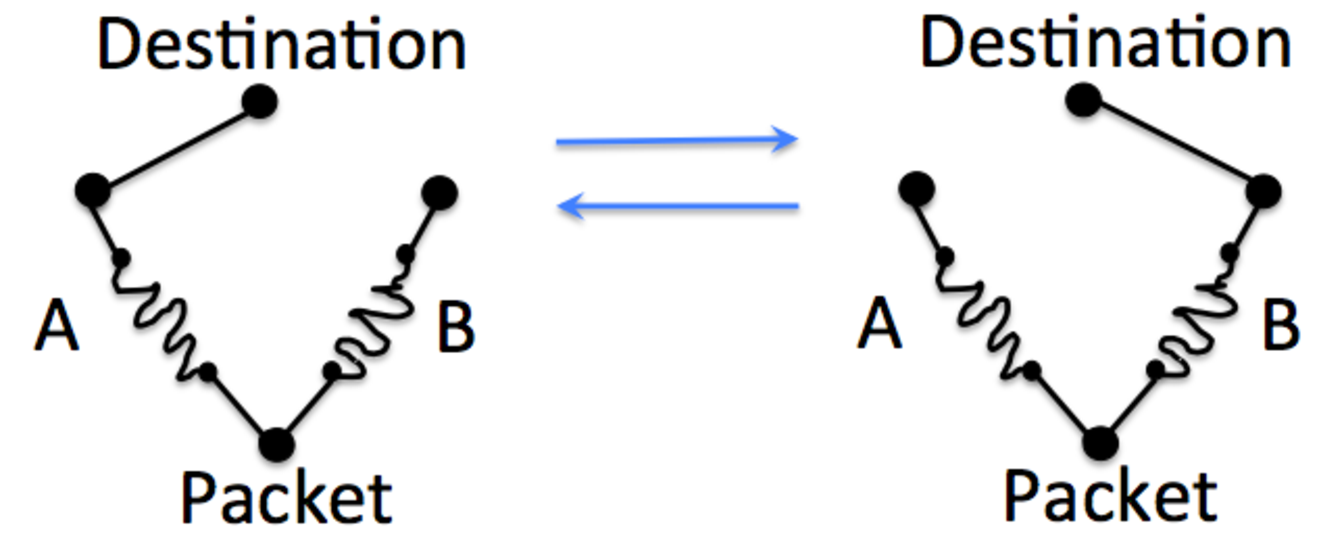
\includegraphics[width=150pt]{PPTFigs/impossible.pdf}
\caption{If the network goes back and forth between the above
  topologies (due to corresponding reconfigurations), then the packet
  will continue to ``swing'' between areas A and B---leading to a
  (perennial) forwarding ``loop''.}
\label{fig:impossible}
\end{wrapfigure}
\para{\underline{(c)} Guaranteeing Bounded Packet Latency.}  The above
strategies still do not guarantee a bounded packet latency. In fact,
in general, its {\em impossible} to guarantee bounded packet latency
(e.g., see Figure~\ref{fig:impossible}). 
%
However, such situations can be avoided if we ensure a minimum time
interval between consecutive reconfigurations; this minimum interval
is also essential for the centralized controlled and the wireless
control channel to be able to handle the resulting load (see
Section~\ref{sec:wireless}.)  In particular, we can formally prove
that a minimum interval of $(x + y)$ time units between
reconfigurations suffices to ensure an upper bound of $2x$ units on
packet latency, where $x$ is the bound on packet latency given a fixed
network and $y$ is the maximum time taken to update (not necessarily
atomically) the network forwarding tables.
%
We can expect $x$ and $y$ to be of the order of 1-2 msecs. Note that
the above claim is independent of the link activation or deactivation
latency (which can be a few tens of msecs).

\para{\underline{(d)} Handling Misalignment of Links.} In \ArchName,
even during a static topology state, links may be temporarily
unavailable because of possible misalignment of the FSO
links. \blue{Such misalignments are fixed in real-time by mechanisms
  suggested in Section~\ref{sec:fso}} in timescales much smaller than
the time needed to update rules~\cite{ddcnsdi13} by an SDN
controller. In fact, it may even be counterproductive to report such
transient link failures to the controller, as it may cause needless
update of forwarding tables. Thus, we need appropriate \blue{network
  layer} techniques to recover from such transient link
failures. \blue{Future SDN roadmaps have provisions for local recovery
  mechanisms analogous to similar schemes in the MPLS and SONET
  literature~\cite{}. We will explore the available alternatives in
  our research. In the absence of such features,} we will investigate
design of a local ``lightweight'' SDN controller on every rack that
can quickly react to such misalignments.


\subsection{A Wire-free Control Channel}
\begin{task} 
\label{task:system:ctrlchannel}
We will design and implement a RF-based  architecture to provide a robust, 
low latency control channel for \ArchName.
\end{task}

\mypara{Problem Context and Challenges} Existing work in the SDN-style
centralized network management literature either implicitly or explicitly
assumes the availability of an ``out-of-band'' control channel that is not
managed by the SDN network itself~\cite{}. This control channel is typically
used for the controller-switch protocols---delivering configuration commands
and collecting switch statistics. Otherwise, there can be subtle bootstrapping
problems with respect to the availability of the control channel itself.
% a problem that is less explored understood in the SDN literature~\cite{}.

%As a starting point for our vision we will assume the existence of an
%out-of-band channel as well. In fact, depending on the deployment scenario this
%might be feasible at very low cost. For instance, using just  2 low-cost 64
%port switches, we can easily connect to $>$ 100  racks per ``container''.

As discussed in the previous section, we will have to engineer a
reliability/consistency mechanism even for the regular inter-rack fabric. We
can exploit this basic reachability framework as a basis for in-band
control. For instance, we can set up static shortest paths between each FSO
switch to the controller at the time of pre-configuration and not reconfigure 
the constituent links. That said, if we are to automate this process, 
we still have a
bootstrapping problem where these switches will need to discover paths to the
SDN controller. Furthermore, there is still a concern  that the control path
may be transiently unavailable during \blue{micro-alignment pauses.} While these may not
be fundamentally intractable, since the reliability of the control 
channel is critical to the operation of the entire network we will explore 
design issues for an out-of-band control channel. 

%Here, we will need to fall back on
%traditional L2/L3 protocols such as STP~\cite{}. (Most commercially available
%SDN switches support a subset of traditional protocols and are not pure
%OpenFlow switches~\cite{}.}


\mypara{Proposed Approach} 
A promising candidate for the out-of-band control
channel is a separate RF-based wireless network in keeping
with the general vision of all-wireless inter-rack fabric. 
%However, commodity wireless technologies may not scale 
%given the needed QoS requirements for 
%the control traffic -- very high link reliability and low latency.
For capacity planning, assume 
%consider the two major types of control traffic: (1) 
%$\approx\!10^{3-4}$ configuration
%change commands per sec from the
%controller to the FSO subsystem on each rack with $\approx\!10^2$ bits per command;
$\approx\!10^3$ new flow arrivals per rack with each 
producing an update of size $\approx\!10^2$ bits to the controller and 
the controller reconfiguring zero or more FSO 
links in response. Further, assume $\approx\!10^3$ 
reconfiguration commands (of size $\approx\!10^2$ bits) from the controller
to the FSO subsystem on each rack. This produces
control traffic comfortably below 1\,Mbps per rack.  Back-of-the-envelop estimates using
dimensions of data center  
and reasonable wireless link budgets show that the
upcoming 802.11ad standard in the 60\,GHz band should be able
to support this rate for about 1000 racks using just 1 channel,
with the controller connected to an AP and with phased-array antennas 
on the controller side (likely to be common for future 802.11ad APs). 
Fixed directional antennas are sufficient
on the racks as they talk to only the controller. 
For larger data centers, multiple channels are needed (supported by multiple
NICs) as the aggregate data rate will push beyond the capacity of a 
single channel. But since at most 3 orthogonal channels are possible
in the 60GHz band, for the largest of the data centers ($\approx\!10,000$ racks),
additional APs ($\approx\,10$, ceiling mounted) distributed across the data center
and connected to the controller via fiber links and a switch
need to be deployed.\footnote{Wires can be completely eliminated
by mesh networking these APs. But since they are very 
few perhaps the added complexity is not worthwhile.} 

The link layer protocol plays an important role to enable
low latency communication. Since the control traffic 
is somewhat regular, scheduled access -- as opposed 
to more conventional CSMA-based random access -- is more meaningful. 
If designed right, this can guarantee a (small) upper bound of the 
channel access delay and a completely interference free channel access. 
Together these properties provide the needed QoS for control
traffic. Note that critical control traffic related
to micro-alignments also go over this control network. This
traffic is expected to be low volume, but should be of the highest
priority. The controller schedules access slots for the clients (racks) based 
the current network state, reconfiguration needs, etc. If multiple
APs are needed for larger systems, interference between 
links is to be pre-determined based on static measurements 
at the setup time. This allows for conflict-free scheduling
of links~\cite{}. Since there is no mobility either at the end points
or in the general RF environment, such measurement-based 
methods are feasible~\cite{}. The 802.11ad standard has support
for scheduled access, so future data centers will be able to 
use commodity RF platforms. However, as many of our
experiences with commodity systems indicate, appropriate software/tool 
support may not be available in commodity systems, e.g., driver-level
and firmware support to implement
special purpose scheduling, measurement support to determine
interference, etc. and it will require working with the device manufacturers. 
Thus, for the purpose of our prototyping, we will custom-build
the RF-based control channel on a software radio platform (USRP/GnuRadio)
in the 2.4\,GHz band\footnote{In a scaled down set up, the 2.4\,GHz band
is enough as the capacity requirement is much lower.} and
implement the scheduling support for demonstration and
evaluation.

% show 
%Direct wireless links from the racks
%to the controller may not scale well at this data rate beyond
%
%
%The capacity requirement per rack is expected to be 
%in the order of 1\,Mbps. To see this, consider i) the 
%control traffic from the controller to the FSO subsystem 
%on the rack -- 
%ii) 
%
%
%A promising alternative to in-band control is to
%equip each ToR switch with a lightweight commodity RF interface. Because the
%bandwidth requirements of this control channel are typically not that high, we
%believe we can use a simple RF-based wireless control channel for the entire
%datacenter. Consider two cases. First, even if we send 1000 configuration
%commands per ToR switch per second, the total bandwidth requirement will be
%less than  {\bf 10 Mbps} per-rack. Second, even if we want to collect per-flow
%statistics per-second from every ToR switch assuming roughly 10K flows/second
%per-rack and assuming a 100 byte flow record size  we will only need {\bf 10
%Mbps} per rack.\footnote{Since the bandwidth demands are low, we could engineer
%a out-of-band channel with a few switches as well. However, this goes against
%our overall vision of a pure wireless network fabric and thus we plan to
%investigate eliminating  this wired control fabric as well.}   
%
%
%The more critical challenge here is {\em latency} of the control channel
%especially for configuration commands. Specifically, if the control loop delay
%is too high then it might induce some stability problems for the
%reconfiguration algorithms as they may not be able to converge in reasonable
%timescales. (Note that we can tolerate some error or delay in the data
%collection or correct for it in the reconfiguration algorithms described
%earlier.) Unfortunately, existing ``commodity'' wireless MAC protocols are not
%geared toward such low-latency.  
%
%
%Because we only need one of these devices per rack, we will design 
% a custom software-radio based  solution using {\bf XXX Samir please fill}
%
% %\vyas{this might be relevant .. but need to think more}

\section{Possible Extensions to \ArchName Architecture}
\label{sec:ext}

In our project, we would also investigate the following ideas, which
impart more flexibility to our design and/or present additional
opportunities to improve \ArchName's performance.

\begin{packeditemize}
\item
{\em Dynamic Reconfiguration of Link Bandwidths.}  In \ArchName, the
\blue{bandwidth} of each FSO link is limited by the capacity of the
ToR switch port. Facilitating FSO links to have variable bandwidth
would add another dimension of flexibility to our design. 
%
This can be achieved by having each port of ToR switch associated with
a unique wavelength, and using a multiplexer and a WSS (wavelength
selective switch) unit between the ToR switch and the FSOs, as in
OSA~\cite{osa-tr}. In essence, the multiplexor and WSS allow one or
more ToR ports to ``feed'' into a single FSO link, and hence,
facilitating variable-bandwidth FSO links. The WSS can be reconfigured
in real-time to determine the allocated ports (and hence, bandwidth)
to each FSO link.
%
It would be interesting and challenging to incorporate the above
flexibility into our design, and appropriately generalize the
techniques from Section~\ref{sec:topology} and~\ref{sec:system}.

\item
{\em Non-ToR Switches and FSOs.} As described before, our network
architecture consists of only ToR switches whose ports are either
connected to the rack machines or the FSOs on the rack. Incorporating
non-ToR switches (as in most data center architectures~\cite{}), whose
ports are connected to only FSOs, can impart more flexibility to
\ArchName's design. The new challenges that need to be addressed in
this context are: (a) Physically accomodating the FSOs connected to
such non-ToR switches in the data center, (b) PCFT, \BBO, and JRTE
problems would include determining the inter-connections between these
additional switches. Note that the resulting PCFT solutions would now
be non-regular graphs.

\item
{\em Vertically Steerable FSOs; $45^\circ$ Mirror Poles.} In our
design, we use a ceiling mirror to circumvent physical obstruction for
line-of-sight FSO communication. However, in certain contexts such as
outdoor scenarios for containerized architectures~\cite{dc-container}
installing a ceiling mirror may not be feasible. In such cases, we
need other mechanisms for line-of-sight communications.  E.g., we can
install FSOs on vertically-steerable poles such that each link
operates on a separate horizontal plane. Another possible mechanism
could be to have FSOs direct their beams to vertically-steerable small
mirrors angled at $45^\circ$. To avoid physical obstruction from
poles/mirrors in the above approaches, shorter distance links can be
operated on a lower horizontal plane than the longer distance links.
\end{packeditemize}

\eat{
\item
{\em Multicast.} Big data applications have diverse communication
patterns that mix together unicast, multicast, all-to-all cast,
etc. Recent works show~\cite{ccr-8} show that all-to-all data exchange
on average accounts for 33\% of the runnign time of Hadoop jobs. As
suggested in~\cite{ccr}, the optical communications are particularly
amenable to efficient implementation of such *-cast patterns by
leveraging various components such as directional couplers,
wavelength-division multiplexed, etc. \blue{Incorporating the above
  ideas in our design will require making challenging design choices.}
}

\newpage
\section{Prototyping and Evaluation Plan}
\label{sec:evalplan}

\begin{task}
\label{task:eval:demo}
We will
evaluate our approach both at an individual  component granularity as well as
an end-to-end prototype and testbed demonstration. 
\end{task}


\begin{packeditemize}

\item {\bf Design and protoype compact, cost-effective, steerable FSO
devices:}  We will prototype a proof-of-concept  10~Gbps SFP-based FSO
devices with a small form factor and design optical mechanisms to
collimate  the laser beam to about 100m.  prototype  two  proposed
steering mechanisms: using switchable mirrors and galvo motors.
%Initially, the design of the collimation and  steering mechanisms will be decoupled
 As a starting point, %To accelerate the initial development of steering mechanisms, 
 we will decouple these two steps and repurpose our existing commodity/outdoor FSO devices~\cite{}
 to test steering mechanisms. 


%As a start, we will begin by using
%commodity platforms~\cite{} and also develop a cost-effective platform for
%tailoring these technologies to the reconfigurable datacenter context. 

\item {\bf Reliability of steerable FSO in realistic conditions:} Real
DCs will  have several sources of ``disturbances'' (e.g., rack
vibration, temperature gradients, airflow patterns, etc.) that may cause
alignment and performance issues for FSO communication.  First, we will
create a  lab environment that can emulate the effects of different
types of disturbances.  To estimate the range parameters for these
effects, we will engage our industry partners (see letters from Facebook
and Microsoft)  and add
instrumentation sensors to compute clusters at local organizations
(e.g., Brookhaven National Lab and CEWIT). Second, we will deploy a
small number of FSO links in an actual DC environment (CEWIT cluster in
Stony Brook University) and conduct a longitudinal study of the
reliability of the links. 

%The final goal of this stage is fine-tuning
%the FSO design via systematic stress-testing and pick one steering
%design for the end-to-end protoyping and evaluation (described
%momentarily). 
 \red{[SD: do we have access to a lab that can emulate ``disturbances"??]}

\item {\bf Performance and benefits under realistic workloads:} We will
develop scalable packet- and flow-level simulation platforms extending
prior work~\cite{htsim,flowsim}  to evaluate the  benefits of our
topology design  (Section~\ref{sec:topology}) and reconfiguration
(Section~\ref{sec:system}) algorithms.  We will start with extrapolating
from existimg small-scale
datasets~\cite{Benson10:IMC,ycsb,ycsb-paper,googleclusterdata} and work
with industry supporters (e.g., Facebook and Microsoft) to quantify the
benefits at scale. 

%ur concepts using real traces.


\item {\bf Responsiveness, and correctness of control plane:}  We will
implement a SDN  controller starting with research prototypes~\cite{pox}
and port our ideas to open-source  platforms such as
OpenDayLight~\cite{} as the project matures.  We will synthesize
benchmark suites to ``stress-test''  the scalability and responsiveness
of our controller.  We  plan to leverage our experiences with emulation
platforms such as MiniNet~\cite{} and Emulab~\cite{} to  test the
correctness of the proposed recovery and consistent reconfiguration
mechanisms in the presence of network dynamics.

\item {\bf End-to-end integration and  evaluation:} A full-scale DC
testbed is outside the scope of the proposal in terms of infrastructure
and personnel resources.\footnote{We plan to develop separate
infrastructure proposals to develop at-scale prototypes.}
%
Within the scope of our budget, we will demonstrate a proof-of-concept
testbed of 4 nodes (node represents a rack). Each node will be
essentially a NetFPGA card~\cite{} on a host computer.  Each NetFPGA
card has 4 x 10G SFP ports, three of which will connect to a FSO device
each with one left for the controller use. We will use OpenFlow switch
implementation on the NetFPGA cards~\cite{} to represent the ToR switch.
 Using NetFPGA will enable precise timing and diagnostic
information~\cite{}, link characterization~\cite{}, as well as aid 
 in high-rate traffic generation~\cite{}.

%Using NetFPGA will allow us use of precise traffic generators for
%repeatable traffic loads~\cite{}, perform very fine-grain, per-hop
%timing measurements and performance analysis in the openflow switch, and
%easy access to the diagnostics information (DOM or digital optical
%monitoring~\cite{}) from the optical SFP for alignment/steering and as
%well as link characterization. \blue{It will also perhaps allow us to
%study innovative packet hadling/forwarding not possible with commodity
%SDN-capable switches.}

The 4 node setup (along with the 4x3=12 FSO devices) will be deployed on
top of the racks in an operational cluster (in CEWIT). %for testing in
realistic environments.  The nodes will be moved around on different
racks to create various geometric possibilities.  This will create
various stress cases for studying the stability of the FSO link and
steering performance. \red{[SD: will somebody complain that real data
centers have real obstructions so such deployment is difficult?]} 

%In
%addition to the characterizing the raw performance of the links, a
%variety of synthetic and trace-driven traffic load will be used to
%evaluate the end-to-end, application perceived performance of the entire
%system. 

%{\bf 4--8} SDN-capable
%switches (e.g., HP Procurve), each configured with {\bf 2-3} FSO-based links
%(e.g., using the commodity galvo meter or mirror design) that can be
%dynamically reconfigured via a central controller running on a server-grade
%platform (e.g., Dell PowerEdge R720 or equivalent).   We will demonstrate the
%viability of reconfigurability at fine-grained timescales as well as the
%(evidently scaled-down) benefits of a flexible architecture.

\vyas{something abt USRP etc?}

\end{packeditemize}


%\mypara{Project Timeline}
%
%\newcommand{\myc}{$\circ$}
%
%\begin{table}[t]
%\begin{center}
%{\small
%\begin{tabular}{l||c|c||c|c||c|c||c|c}
%		& \multicolumn{2}{c||}{Year 1 (2014)} & \multicolumn{2}{c||}{Year 2 (2015)} & \multicolumn{2}{c||}{Year 3 (2016)}  & \multicolumn{2}{c}{Year 4 (2017)}\\
%					& Fall & Spring & Fall & Spring & Fall & Spring & Fall & Spring \\ \hline
% \taskref{task:system:fastalgo}: Algorithms 	&	&  & & \myc &  \myc  &       \myc   & \myc &  \\
% \taskref{task:system:dataplane}: DataPlane 	&	&  & & \myc &  \myc  &       \myc   & \myc &  \\
% \taskref{task:system:ctrlchannel}: ControlChannel 	&	&  & & \myc &  \myc  &       \myc   & \myc &  \\
% \taskref{task:eval:demo}: E2E Demos 	&	&  & & \myc &  \myc  &       \myc   & \myc &  \\
%\end{tabular}
%}
%\end{center}
%\vspace{-0.5cm}
%\tightcaption{Projected schedule for tasks described in the previous sections. The $\circ$ shows when 
% a task is ``active''.  Some tasks are  split in the timeline as we 
% will need to revisit/integrate with respect to other aspects of the proposed work. 
% }
%\vspace{-0.5cm}
%\label{tbl:schedule}
%\end{table}
%

\section{Broader Impact}
\label{sec:edu}

\red{Some input from Jon would be helpful too.}

\para{Impact on Economy and Environment.} 
With growing interest in
Big Data, cloud computing and virtualization, data centers are now
common in every sector of the economy. This includes IT industry,
government, media, healthcare, financial sector, transportation
and the scientific community. 
The largest of the data centers are known to cost more than a billion USD
and are significant power hogs consuming 10s of MW of power~\cite{}. 
Overall, recent EPA studies concluded the the total data center electrical power usage is 
roughly a few percent of the entire electricity consumption in the US
and lagging only modestly behind the total household electricity consumption~\cite{}. 
We foresee that the Firefly architecture can significantly reduce both cost 
(by eliminating the need for over-provisioning)  
and energy consumption (by making the network design
energy-proportional and also by improving cooling). 
This certainly will have perceptible economic impact by making many
IT services cost less - both in terms of dollars and carbon footprint - across all sectors in the economy. 
In addition, success in the proposed project will garner immediate interest in industry 
for further developing and productizing the proposed FSO-based interconnection.
R\&D and manufacturing of such interconnections will produce 
a different form of device industry that will include optical engineers
in addition to traditional computer hardware engineers. 


%
%Performance of data centers, energy savings
%(energy proportionals DCs), cabling complexity, broaden the current
%applications of FSO communication (which is currently limited to specialize
%across-town applications), ad hoc deployment of interconnection architectures 
%(e.g, for Helios type containerized DCs), 

\paragraph{Integration of Research and Education.}

 A strength of the project is that it brings together two disparate disciplines,
opto-electronics and computer systems. 
Due to this unique nature, the participating ME students will learn
basics of data center networking and the CS students will be exposed
to laser communications. From
preliminary studies leading to this proposal -- that involved several grad students from both CS and ME -- 
it is our experience that 
the students particularly enjoyed learning a completely
new technology and understanding the methods and practices of a
different discipline. 

The project will 
directly contribute to relevant graduate courses in both mechanical engineering (ME) and
computer science (CS) that the PIs teach regularly. These include
advanced courses on ``wireless networking'' (Gupta/Das), 
``software-defined networking'' (Sekar) and core graduate
courses in ``networking'' (Sekar/Das). The PIs regularly 
scope out suitable topics from their existing research projects
to assign term projects to these graduate level classes. Over the past
years, such projects motivated students better due to their
direct contribution to a bigger effort. This improved participation
as well as the final results, often students continuing working on these topics past the 
course term, writing papers or developing various
 artifacts of longer term value. 

%especially by having  relevant project topics and lab support
%available to the students. We also plan to develop tutorial materials 
%on data center networking and FSO communications, present such 
%tutorials in relevant conferences and finally make them available freely
%via YouTube. 

%\vyas{probably need some concrete pointers here on wireless classes,
%SDN/advanced classes, theory classes etc that we have taught and generated some
%tangible research from}
%
%\samir{addressed.}

\para{Engaging High School and Undergraduate Students.}  Long Island
have some of the best public schools in the country and we are keen on
tapping into this high school talent. SBU has a Simons Summer
Research Program\footnote{\normalsize
  http://www.stonybrook.edu/simons/} that provides a mechanism to
recruit talented high school students.  PIs Gupta and Das
have mentored students in the past in this program whenever
they had projects that high schooler could relate to easily (e.g.,
on RFID tracking and robot navigation). 
The proposed project brings in `hands-on' components
such as FSO  communications, use of steerable lasers to implement
network switching that we believe would be of interest to the
participating high schoolers in the Simons program. 
We hope to be able to recruit 1-2 such students each summer. 
% Students in the this program routinely competes
%nationally in the Intel Science
%Talent Search and often successfully with SBU professors as mentors. 
%
%During the past few summers at SBU, our colleagues have also organized
%Engineering Camps to attract high school students to come to SBU; At
%the camps, the students have several two-day laboratories in which
%they are instructed on how to design, build, and program various types
%of devices.
%%
%The above programs would provide perfect avenues to recruit a few
%high-school students for summer projects related to our research.


The PIs have strong history of involving undergraduates
in research and supporting them via REU supplements. This
approach motivated a few of them enough in the past
that they joined in the graduate program. The PIs
will continue this involvement for the proposed project.

%Due to the hi-tech appeal of free-space optics in data communications
%and other applications, we are keen on giving presentations and
%demonstrating appropriate aspects of our research prototype to some
%high-schools and our undergraduate students. We believe that the
%obvious appeal of free-space optics and steering mechanisms will be
%exciting for the students, and give us an opportunity to further
%encourage and recruit some of the best students.
%%
%Finally, we plan to build ``kits'' that can be used by the students to
%build hobby projects, e.g., FSO-based scanning devices, inexpensive
%custom-built steering mechanisms for FSO devices, demonstration of
%high-bandwidth FSO links using commodity hardware, etc. More elaborate
%projects based on the above ideas would be ideal for senior projects. 
%
%We hope to motivate them high-school students to pursue further
%education and careers in computer science. Many of the Simons Summer
%Research Program participants have excelled at the Intel Science
%Talent Competition (ISTC), and we are keen on mentoring high school
%students for ISTC.

%\vyas{is there concrete evidence .. this seems to say someone else in SB has done this, not necessarily us :) }
%
%\vyas{are the kits budgeted for?}

\para{Involving Under-Represented Groups.} 
The PIs have history of mentoring students
from the traditionally under-represented groups
in STEM disciplines. Gupta and Das has graduated
a woman PhD student each in the recent past and Das currently advises
one woman PhD student. Earlier, Das also graduated
a PhD student, Robert Casta\~{n}eda, from the Hispanic community and 
Casta\~{n}eda is currently 
a faculty member in a minority serving college in his native San Antonio. 
Das also served in several related NSF organized outreach efforts, e.g., mentoring faculty from minority-serving institutions
for writing competitive NSF grants. The PI will continue similar efforts
in connection with the proposed project. 

%SBU has a
%history of active outreach efforts in order to involve traditionally
%under-represented groups in science and engineering research. 
%This includes the Turner Fellowship Program minority
%for graduate students, the SUNY Alliance for Minority Participation (SUNY AMP), a
%minority faculty recruitment initiative, and the SUNY Alliance for
%Inclusive Graduate Education and the Professoriate (SUNY AGEP).
%Research in undergraduate studies will also be integrated through the
%\emph{Women In Science \& Engineering (WISE)} mentoring program in
%SBU, which regularly offers four-week research and inquiry-based
%courses. We plan to introduce a new WISE course related to free-space
%optics communications and applications. The PIs are committed to
%involve under-represented groups in ``high-tech'' research and
%development.

%\vyas{probably should say something abt pis track record in working
% with underrepresented gro?}


\section{Results From Prior NSF Support}

\textbf{Samir R. Das} and \textbf{Himanshu Gupta} are PI/Co-PIs on the following 
recently concluded/ongoing NSF awards:
%i) `A Measurement-Driven Physical-Interference-Based Approach for the Design of Mesh Networks' (2007-09, \$200,000), 
i) `A Market-Driven Approach to Dynamic Spectrum Sharing' (2008-13, \$406,000), and  ii) 
`Understanding Traffic Dynamics in Cellular Data Networks and Applications to Resource Management,' (2011-14, \$320,425).  
%The first award resulted in developing measurement-driven methodologies for understanding wireless 
%interference and exploiting them for transmission scheduling. 
%
These projects
focus on developing market-driven algorithms and systems for dynamic spectrum access systems (first)
and understanding spatio-temporal traffic dynamics in cellular data networks via analysis of network traces and using them
for spectrum/energy management applications (second). Over 15 papers were co-authored by the PIs 
related to these awards and 6 PhD students received
direct support. The PIs gave several public lectures based on the results.
%\red{[SD: if we have space we may also mention the sensor grants.]}. 
%and taught well-received 
%tutorials (on mesh networks and on interference modeling). 
%The awards
%also contributed to developing teaching materials in graduate and undergraduate wireless networking class
%that the PI teaches and generated
%or strengthened industry collaborations (NEC Research, Bell Labs and start-ups).

\textbf{Jon Longtin}, Co-PI, CBET-1048744, ``NSF/DOE Thermoelectrics Partnership:
Integrated Design and Manufacturing of Cost-Effective and
Industrial-Scalable TEG for Vehicle Applications,'' \$404,226,
10/1/10-09/30/13. This work developed thermoelectric materials and systems
for automotive applications using thermal spray technology. $\mathrm{Mg_{2}Si}$ and
filled Skudderudites were deposited directly onto exhaust system
components to convert exhaust waste heat to electricity. Key tasks on the
project included 1) materials development and characterization, 2)
short-pulse laser micromachining deposited thermoelectric materials, 3)
techniques for fabrication of multi-layer thermoelectric generators, and
4) device characterization and testing.  6 conference, 4 journal
publications, 4 Masters thesis and 1 Ph.D. thesis have resulted from the
project.


%% VS: not sure what to say here .. it has cloud in the title so i do want to say something to distance it and also say that i cant have anything to show since it just got funded
\textbf{Vyas Sekar} is a PI on two recently awarded NSF grants ``Enabling
Flexible Middlebox Processing in the Cloud'' and ``Rethinking Security in the
Era of Cloud Computing'' starting in Sep 2013. The research proposed therein
focuses largely on ``middlebox'' functionality such as IDS, firewall, and
proxies and does not focus on the datacenter topology and routing aspects.
These projects have just commenced and there are no outputs at this time.  As
such the proposed research in these projects does not overlap with the
management layer/SDN approaches proposed here. 



{
\bibliographystyle{plain}
\bibliography{../bib/Ref,../bib/VyasRef}
}

\end{document}
